\documentclass[11pt]{article}
\usepackage{geometry}                % See geometry.pdf to learn the layout options. There are lots.
\geometry{letterpaper}                   % ... or a4paper or a5paper or ... 
%\geometry{landscape}                % Activate for for rotated page geometry
\usepackage[parfill]{parskip}    % Activate to begin paragraphs with an empty line rather than an indent
\usepackage{graphicx}
\usepackage{amssymb}
\usepackage{amsmath}
\usepackage[normalem]{ulem}
\usepackage{epstopdf}
\usepackage{bm}
\usepackage{float}
\restylefloat{figure}
\usepackage{titlesec}
\usepackage{verbatimbox}
\usepackage{multicol}
\usepackage{multirow}
\usepackage{caption}
\usepackage{empheq}
\usepackage{hyperref}
\usepackage{tikz}
\captionsetup{skip=0pt}
%\renewcommand{\baselinestretch}{1.2}


\newcommand{\tallrow}{\phantom{$\displaystyle\frac{\sum}{\sum}$}}


\DeclareGraphicsRule{.tif}{png}{.png}{`convert #1 `dirname #1`/`basename #1 .tif`.png}
\pagestyle{plain}
%\setcounter{page}{179}
\newcommand{\ub}[1]{{\bf \uline{#1}}}
\newcommand{\ds}{\displaystyle}


\setlength{\textwidth}{6.5in}
\setlength{\oddsidemargin}{-.25in}
\setlength{\evensidemargin}{-.25in}
\setlength{\textheight}{9.0in}
%\setlength{\topmargin}{-0.5in}
\setlength{\topmargin}{-.7in}
%\setlength{\oddsidemargin}{-.25in}
%\setlength{\evensidemargin}{-.25in}
%\pagestyle{headandfoot}
%\firstpageheader{Stat 341}{Survey of Statistical Methods}{}


%\title{Brief Article}
%\author{The Author}
%\date{}                                           % Activate to display a given date or no date

\begin{document}
\large
\begin{center} \fbox{\Large{\bf Notes 8: Bayesian Methods}} \end{center}

All of the statistical inference you have learned up to this point has been in the \ub{frequentist} framework. In this view, all \uline{parameters are fixed numbers} and we use methods to try to determine what those numbers are. We do not associate probabilities with parameters, but we can establish the probability that our inferential procedures are correct. All of the hypothesis testing (even the nonparametric tests) and confidence intervals we have dealt with are frequentist inference methods. 

However, there is an entire other paradigm that many statisticians have adopted known as the \ub{Bayesian} framework, named after Thomas Bayes who lived in the 18th century and the theorem he developed. In Bayesian statistics, \uline{parameters are viewed as random variables} that have probability distributions. If we know that the probability distribution is for a parameter, we can simply obtain random samples from that distribution to perform inference. Bayesian statistics is becoming increasingly popular and is especially useful in \ub{uncertainty quantification} in statistics and other fields.\\

To get an idea of how Bayesian statistics works, let's first discuss conditional probability and Bayes' Theorem. 

\fbox{\bf Conditional Probability and Bayes' Theorem}

\begin{minipage}{.475\textwidth}
\href{bayes_figs/https://imgs.xkcd.com/comics/conditional_risk.png}{xkcd comic}\\
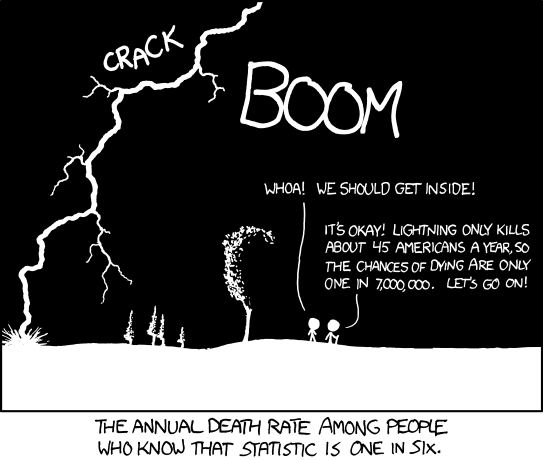
\includegraphics[width = 2.5in]{bayes_figs/conditional_risk.png}
\end{minipage}
\hfill
\begin{minipage}{.5\textwidth}
As suggested in the comic to the left, probabilities can change based on the condition that another event has occurred. For example, what is the probability that a randomly chosen man is over 6 feet tall? About .14. What is that same probability given that you are selecting from an NBA basketball team? Almost 1. The probability changes given the fact that you are selecting from a basketball team.
\end{minipage}
%\noindent \underline{Example}: In a study of suicide victims between 2000-2017, \\ it was
%found that 79\% were male, 52\% were committed by \\ firearm, and 44\% were males who used
%a firearm.
%
%\vspace{0.2in}
%\noindent Let: \\ % $M$ = event that the victim was male,
%
%%\noindent \hspace{0.24in} $F$ = event that the victim used a firearm.
%\vspace{-1.8in}
%\begin{figure}[H] \hspace{4.0in}
%\psfig{figure=Postscript/emptyVenn.ps,height=2.2in,width=2.8in}
%\end{figure}
%
%\vspace{0.0in}
%\noindent (a) What is the probability a randomly chosen victim was female AND used a firearm?
%\\ \\ \\
%%\begin{eqnarray*}
%%P(M^{c}F) = .09 = P(F) - P(MF) = .59 - .50.
%%\end{eqnarray*}
%\noindent (b) \underline{Given that the victim is male}, what is prob. he used a firearm?
%
%\hspace{0.1in} $\rightarrow$ Given \underline{extra} info here - so the probability
%is \underline{conditional} on this extra info.
%\begin{itemize}
%\item From Venn: %prob = \(\displaystyle{\frac{.50}{.28+.50} = \frac{.50}{.78}} =
%%\underline{.64} > .59 \;\;\) (Prob. of using a firearm).
%\item So the extra info \underline{changed} (and in fact increased) the prob. of using a
%firearm.
%\end{itemize}
\vspace{.2in}

\noindent
{\bf Example: Medical Testing}. A disease affects 0.1\% of the population. The medical test for this disease can be described as 95\% accurate. If you test positive, what is the chance you have the disease?\\ 
\vspace{2cm}

\newpage

%\noindent \underline{Example}: Suppose we roll a fair dice twice, recording the value each time.  Note that the
%sample space for this experiment can be written as below, where ``ab'' indicates
%an ``a'' on the 1st roll and a ``b'' on the 2nd roll.
%\begin{eqnarray*}
%\hspace{3.9in} S = \left\{ \begin{array}{cccccc} 11 & 12 & 13 & 14 &
%15 & 16 \\ 21 & 22 & 23 & 24 & 25 & 26 \\ 31
%& 32 & 33 & 34 & 35 & 36 \\ 41 & 42 &
%43 & 44 & 45 & 46 \\ 51 & 52 & 53 & 54 &
%55 & 56 \\ 61 & 62 & 63 & 64 & 65 & 66
%\end{array} \right\}
%\end{eqnarray*} \vspace{-1.4in}
%
%\begin{enumerate}
%\item[(a)] What is the probability that we roll two sixes? \\ \\ \\ \\ \\
%\item[(b)] What is the probability that we roll two sixes\\
%if we know the first die roll was a 6? \\ \\ \\ \\ \\ \\ 
%\item[(c)] What is the probability that we roll two sixes if we know at least one of the die rolls was a 6?
%\vspace{.8in}
%\end{enumerate}

%\noindent
%{\bf Example: Amos Tversky and Daniel Kahneman taxicab problem (1982).}      A cab was involved in a hit and run accident at night. Two cab companies, the Green and the Blue, operate in the city. 85\% of the cabs in the city are Green and 15\% are Blue.
%
%\noindent A witness identified the cab as Blue. The court tested the reliability of the witness under the same circumstances that existed on the night of the accident and concluded that the witness correctly identified each one of the two colors 80\% of the time and failed 20\% of the time.
%
%\noindent What is the probability that the cab involved in the accident was Blue rather than Green knowing that this witness identified it as Blue? In other words, what percentage of cars identified as Blue are actually Blue?
%
%\vspace{2in}
%\noindent
%P(random cab is Blue) = .15. \\
%P(random cab is Blue given that it has been identified as Blue by witness) = .41.\\
%This is a {\it conditional probability}. Notation: separate the event from the condition with $|$.


\noindent \underline{Definition}:  If $A$ \& $B$ are any events with $P(B)>0$,
then the \underline{\bf conditional}

\hspace{0.70in} \underline{\bf probability of $A$ given that $B$ occurred} is:
\begin{eqnarray*}
\fbox{\(P(A|B) = \displaystyle{\frac{P(A\cap B)}{P(B)}}\)} \;\; {\mbox{ ``prob of $A$
given $B$''}}.
\end{eqnarray*}
%\begin{itemize}
%\item In the example, we want \(\underline{P(F|M)} = \)%\displaystyle{\frac{P(FM)}
%%{P(M)} = \frac{.50}{.78}} = \underline{.64} \neq .59 = P(F)\).
%\end{itemize} \vspace{0.1in}

%\newpage
\noindent \underline{Example}:  Roll fair die 3 times ($6^{3} = 216$ total
outcomes in $S$). \\ Let $A$ = event that sum is 4 or less, so $A$ = \\
%$\{111,112,121,211\}$
Let $B$ = event that first roll is even.  What is
$P(A|B)$? \\ \\ \\ \\ \\ \\
%\begin{eqnarray*}
%P(E|F) = \frac{P(EF)}{P(F)} = \frac{1/216}{108/216} = \frac{1}{108} \left[
%\begin{array}{c} {\mbox{Of all 108 events in }} F, {\mbox{ only}} \\ {\mbox
%{1 of them is in }} E \end{array} \right].
%\end{eqnarray*}
%\hspace{2.0in} $\longrightarrow$ (\# outcomes in $F$: \underline{3} $\cdot$
%\underline{6} $\cdot$ \underline{6} = 108)
\begin{itemize}
\item $B$ can be viewed as a restricted sample space (i.e.: we know the
outcome is in $B$, now what is prob. it is also in $A$?).
%\item What is $P(E|F^{c})$?  = %\(\displaystyle{\frac{P(EF^{c})}{P(F^{c})} =
%\frac{3/216}{108/216} = \underline{\frac{3}{108}}}\).

%\vspace{0.1in} (since 3 outcomes in $E$ have first roll being odd.)
\end{itemize}

%\vspace{0.2in}
%\noindent \underline{Are conditional prob's really prob's?} - What does it
%mean to say this? \\ (i.e.: - Does $P(\cdot|F)$ satisfy Kolmogorov's Axioms?)
%\vspace{1.5in}

%\vspace{-0.2in}
%\begin{figure}[H] \hspace{1.04in}
%\begin{picture}(100,25)(0,0)
%\put(0,25){\line(0,-1){19}} \put(1,6){\oval(2,2)[bl]}
%\put(2,4){\vector(1,0){18}} \put(22,0){\small indicates what $P$ is function
%of} \put(10,25){\line(0,-1){6}} \put(11,19){\oval(2,2)[bl]}
%\put(12,17){\vector(1,0){8}} \put(22,13){\small $F$ is fixed}
%\end{picture} \end{figure}

%\begin{itemize}
%\item They do satisfy Kolmogorov's Axioms, so conditional prob's are prob's,
%and hence satisfy all probability theorems (**) [Section 3.5 in the text.] 
%
%\noindent
%\underline{Ex}: $P(E^{c})=1-P(E) \Rightarrow P(E^{c}|F) = 1-
%P(E|F)$\\ \\
%\hspace{1in} \underline{Ex}: Inclus/Exclus: $P(E_1\cup E_2|F) = P(E_1|F)+P(E_2|F) - P(E_1\cap E_2 |F)$.\\ 
%
%\underline{Ex}: Partitions: $P(E|F)=\sum_{i=1}^\infty P(E\cap S_i|F)$ where $S_1,S_2,\dots$ is a partition of $S$.\\
%\end{itemize}
%
%\noindent \underline{Note}: Since \(P(E|F) = \displaystyle{\frac{P(EF)}{P(F)}}
%\) and \(P(F|E) = \displaystyle{\frac{P(EF)}{P(E)}}\), then:
%\begin{center} \underline{$P(EF) = P(E|F)P(F) = P(F|E)P(E)$}. \hspace{0.2in}
%{\bf (Useful Identity)} \end{center}
 
% \newpage
%\vspace{0.1in}
%\noindent \underline{Example}: Randomly choose a student at a certain school. \\ Suppose
%60\% of the students are female, and 20\% of the \\ females are English majors. \vspace{-1.1in}
%\begin{figure}[h] \hspace{4.0in}
%\includegraphics[width = 2.8in, height = 2.2in]{emptyVenn.pdf}
%\end{figure} \vspace{-1.4in}
%
%\noindent (a) What is the probability you choose a female \\ English major? \\ \\ \\ \\
%
%%\vspace{0.1in}
%%\( \left. \begin{array}{rl} {\mbox{Let }} F = & {\mbox{event the selected
%%person is female,}} \\ E = & {\mbox{event the selected person is an English major}}
%%\end{array} \right\} \;\;\) Want $P(EF)$.
%
%%\vspace{0.1in}
%%$P(F)=.60$ (unconditional prob.).  What is $.20$? = $P(E|F)$.
%
%%\vspace{0.1in}
%%So the prob. we choose a female English major is: \[P(EF) = P(E|F)P(F) = (.20)(.60)
%%= \underline{.12}.\]
%
%\vspace{0.2in}
%\noindent (b) Suppose 15\% of the students are English majors.  Given that we
%choose an English major, what is the probability she is female? \\ \\ \\ \\ \\
%%\begin{itemize}
%%\item Given: $P(F)=.60, P(E|F)=.20, P(E)=.15$.
%%\item Want: $P(F|E)$.  By the note:
%%\begin{eqnarray*}
%%P(E|F)P(F) & = & P(F|E)P(E) \Leftrightarrow (.20)(.60) = P(F|E)(.15) \\ &
%%\Leftrightarrow & \underline{P(F|E)} = \frac{(.20)(.60)}{.15} = \frac{.12}{.15}
%%= \underline{.80}.
%%\end{eqnarray*}
%%\end{itemize}
%%
%%\vspace{0.1in}
%%\noindent \underline{Example}:  Suppose in manufacturing  20 soccer balls, 4
%%have defective stitching.
%%
%%\vspace{0.1in}
%%\noindent (a) If we randomly select 2 balls w/o replacement, what is the probability
%%that neither have defective stitching? \\ \\ \\ \\ \\  %\hspace{3.7in} One way:
%%
%%%\vspace{-0.4in}
%%%\begin{eqnarray*} \hspace{4.6in} \left[ \frac{\small
%%%\left( \begin{array}{c} 16 \\ 2 \end{array} \right)}{\small \left(
%%%\begin{array}{c} 20 \\ 2 \end{array} \right)} = \frac{\frac{16 \cdot 15}{2}}
%%%{\frac{20 \cdot 19}{2}} = \frac{12}{19}. \right]
%%%\end{eqnarray*}
%%%\vspace{-0.9in}
%%%\begin{itemize}
%%%\item Let $B_{1}$ = event the 1st ball is not defective,
%%
%%%\hspace{0.25in} $B_{2}$ = event the 2nd ball is not defective.
%%%\item Want \underline{$P(B_{1}B_{2})$} = $P(B_{1})P(B_{2}|B_{1})$ =
%%%\(\displaystyle{\frac{16}{20} \cdot \frac{15}{19} = \underline{\frac{12}
%%%{19}}}\).
%%%\end{itemize}
%%
%%\noindent (b) If we randomly select 4 balls w/o replacement, what is prob.
%%that none have defective stitching? \\ \\ \\ \\ \\ \\ \\ \\ %\hspace{4.4in} One way:
%%
%%%\vspace{-0.4in}
%%%\begin{eqnarray*} \hspace{4.6in} \left[ \frac{\small
%%%\left( \begin{array}{c} 16 \\ 4 \end{array} \right)}{\small \left(
%%%\begin{array}{c} 20 \\ 4 \end{array} \right)} = \frac{\frac{16 \cdot 15
%%%\cdot 14 \cdot 13}{4!}}{\frac{20 \cdot 19 \cdot 18 \cdot 17}{4!}}. \right]
%%%\end{eqnarray*}
%%%\vspace{-0.9in}
%%%\begin{itemize}
%%%\item Let $B_{3}$ = event the 3rd ball is not defective
%%
%%%\hspace{0.29in} $B_{4}$ = event the 4th ball is not defective.
%%%\end{itemize}
%%%\begin{eqnarray*}
%%%P(B_{1}B_{2}B_{3}B_{4}) & = & P(B_{1}) P(B_{2}|B_{1}) P(B_{3}|B_{1}B_{2})
%%%P(B_{4}|B_{1}B_{2}B_{3}) \\ & = & \frac{16}{20} \cdot \frac{15}{19} \cdot
%%%\frac{14}{18} \cdot \frac{13}{17} = \underline{\frac{364}{969}}.
%%%\end{eqnarray*}
%%
%%\vspace{0.1in}
%%\noindent General Result: \underline{\bf Multiplication Rule}:  For any events
%%$E_{1}, \ldots, E_{n}$:
%%\begin{eqnarray*}
%%P(E_{1}E_{2} \cdots E_{n}) = P(E_{1}) P(E_{2}|E_{1}) P(E_{3}|E_{1}E_{2})
%%\cdots P(E_{n}|E_{1}E_{2} \cdots E_{n-1}).
%%\end{eqnarray*}
%%
%%\vspace{0.2in}
%%\noindent \underline{Proof}: \underline{RHS} = 
%%%\(P(E_{1}) \cdot \displaystyle
%%%{\frac{P(E_{1}E_{2})}{P(E_{1})} \cdot \frac{P(E_{1}E_{2}E_{3})}{P(E_{1}E_{2})}
%%%\cdots \frac{P(E_{1} \cdots E_{n})}{P(E_{1} \cdots E_{n-1})}} = \underline
%%%{P(E_{1} \cdots E_{n})}\).
%
%%\vspace{0.8in}
%\noindent \underline{Example}:  Consider modeling stock market movement.  Suppose:
%
%the prob. the stock index $\uparrow$ today given it went $\downarrow$
%yesterday = .4
%
%the prob. the stock index $\uparrow$ today given it went $\uparrow$
%yesterday = .7
%
%the prob. the stock index $\downarrow$ today given it went $\downarrow$
%yesterday = %.6
%
%the prob. the stock index $\downarrow$ today given it went $\uparrow$
%yesterday =% .3
%
%\vspace{0.2in}
%\noindent \underline{Note}:  With this model, we \underline{only} need to
%know what happened the \underline{previous} day.
%\begin{itemize}
%\item Let $E_{i}$ = event the stock index went up on day $i$, $i=1,2,\ldots$.
%\item So $P(E_{i}|E_{i-1}) = .7, P(E_{i}|E_{i-1}^{c}) = .4, P(E_{i}^{c}|
%E_{i-1}) = .3, P(E_{i}^{c}|E_{i-1}^{c}) = .6$, $\forall i$.
%\end{itemize}
%
%\noindent Suppose on day 1, the index went up.  What is the prob. it goes
%down on days 2 \& 3 and then back up on day 4? 
%\vfill
%
%%\begin{eqnarray*}
%%\underline{P(E_{2}^{c}E_{3}^{c}E_{4}|E_{1})} & = & P(E_{2}^{c}|E_{1}) \cdot
%%P(E_{3}^{c}|E_{1}E_{2}^{c}) \cdot P(E_{4}|E_{1}E_{2}^{c}E_{3}^{c}) \;
%%{\mbox{(Mult. Rule)}} \\ & = & P(E_{2}^{c}|E_{1}) \cdot P(E_{3}^{c}|E_{2}^{c})
%%\cdot P(E_{4}|E_{3}^{c}) \; {\mbox{(by Note)}} \\ & = & (.3)(.6)(.4) =
%%\underline{.072}.
%%\end{eqnarray*}
%\begin{itemize}
%\item This type of process is known as a \underline{\bf Markov chain}, which is
%characterized by the note above. (i.e.: Only need to know immediate past.)
%\end{itemize}


\vspace{0.2in}
\ub{Bayes' Theorem }

\noindent \underline{\bf Useful Result}:  For any events $A$ and $B$: %(where $0<P(B)<1$):
\begin{eqnarray*}
\underline{P(B)} & = & P((A\cap B) \cup (A^c\cap B)) = P(A\cap B) + P(A^c\cap B)\\
& = & \underline{P(B|A)P(A) + P(B|A^{c})P(A^{c})} \;\;
{\mbox{(using the definition of conditional  prob.)}}.
\end{eqnarray*}

\noindent \underline{Example}: \underline{(False positives)}: For pregnant women over age 35, doctors often recommend a test for Down
syndrome early in the second trimester. This is due to a higher risk of having a child with Down syndrome. One test screens for the presence of alpha fetoprotein (AFP) in the mother's blood. This test is somewhat
controversial because of its high \underline{\bf false positive} rate.
\begin{itemize}
\item When this test is given to a mother of age 36, the probability that:
\begin{itemize}
\item the test is positive when there is a baby with Down syndrome is 0.999,
\item the test is positive when there is not a baby with Down syndrome is 0.05,
\item the test is negative when there is a Down syndrome baby is
\item the test is negative when there is not a Down syndrome baby is
\end{itemize}
\end{itemize}
\noindent Problem: some women are told they have a Down syndrome baby when they don't
(false positive).
\begin{itemize}
\item Suppose 1 of every $400$ babies born to mothers over the age of 35 have
Down syndrome.
\item Given that the AFP test is positive, what is the probability a randomly
chosen mother of this age has a Down syndrome baby?
\item Let: \\ \\% $T$ = event the test is positive,

%\hspace{0.28in} $C$ = event a randomly selected person has cancer type.
\item Know: \\ \\%\( \begin{array}{cc} P(T|C)=0.95, & P(T|C^{c})=0.05 \\
% P(T^{c}|C)
%=0.05, & P(T^{c}|C^{c})=0.95 \end{array}\) \& \(P(C) = \frac{1}{100000} =
%0.00001\).
\item Want: \\ \\ \\ \\
\end{itemize} %\vspace{-0.2in}
%\begin{eqnarray*}
%{\mbox{Want }} \underline{P(C|T)} & = & \frac{P(CT)}{P(T)} = \frac{P(T|C)P(C)}
%{P(T|C)P(C) + P(T|C^{c})P(C^{c})} \;\; {\mbox{(by Useful Fact)}} \\ & = &
%\frac{(.95)(.00001)}{(.95)(.00001) + (.05)(.99999)} = \frac{.0000095}{.050009}
%= \underline{.00019}.
%\end{eqnarray*}
\begin{itemize}
\item So there is a \underline{\hspace{0.5in}} chance of having a Down syndrome baby
when the mother tests positive!
\item What happened here?  With only 1 in 400 having Down syndrome, in every
400 babies, we expect: \underline{1} to have Down syndrome \& nearly \underline{20}
to test positive w/o Down syndrome (5\%).
\item Your chances of being in the false positive group are \underline{much}
higher.
\item Another way to solve this problem is with a \underline{tree diagram}:

\begin{figure}[H] \begin{center}
\begin{picture}(450,265)(0,0)
%\put(0,0){\framebox(450,265)}
\put(0,135){\line(1,1){80}} \put(0,135){\line(1,-1){80}}
\put(85,215){syndrome}\put(85,225){Down} \put(85,45){syndrome} \put(85,55){No Down}
\put(135,217){\line(2,1){80}} \put(135,217){\line(2,-1){80}}
\put(135,47){\line(2,1){80}} \put(135,47){\line(2,-1){80}}
\put(220,255){Positive} \put(220,172){Negative}
\put(220,85){Positive} \put(220,3){Negative}
\end{picture} \end{center} \end{figure} \vspace{1.0in}
\end{itemize}

\vspace{-1in}
\noindent \underline{\bf General Useful Result}:  Let $B$ be any event in the sample space $S$ and
let $A_{1}, \ldots, A_{n}$ form a partition (disjoint) of $S$, with $P(A_{i})>
0$.  Then $B = (B\cap A_{1}) \cup (B\cap A_{2}) \cup \cdots \cup (B\cap A_{n})$, a disjoint
union since $F_{i}$'s are disjoint.
\begin{eqnarray*}
{\mbox{So: }} \; \underline{P(B)} & = & P \left( \bigcup_{i=1}^{n} B\cap A_{i}
\right) = \sum_{i=1}^{n} P(B\cap A_{i}) \\
& = &
\underline{\sum_{i=1}^{n} P(B|A_{i})P(A_{i})}.
\hspace{4.0in}
\end{eqnarray*}

\vspace{0.1in}
\noindent \underline{{\bf Bayes Theorem (in discrete case)}}:  Let $A_{1}, \ldots,
A_{n}$ partition $S$, so that $P(A_{i})>0$ for $i=1, \ldots, n$ and let $B$
be any event such that $P(B)>0$.  Then for each $i=1, \ldots, n$:
\begin{eqnarray*}
P(A_{i}|B) = \frac{P(A_i\cap B)}{P(B)}= \frac{P(B|A_{i})P(A_{i})}{P(B)}  = \frac{P(B|A_{i})P(A_{i})}{\sum_{j=1}
^{n} P(B|A_{j})P(A_{j})}.
\end{eqnarray*}

\noindent \underline{Example}: A hospital receives 40\% of its flue vaccine from Company A, 50\% from Company B, and the rest from Company C. From Company A, 3\% of its vaccine doses are ineffective, from Company B, 2\% are ineffective, and from company C, 4\% are ineffective.  Given a randomly chosen doses is ineffective, what is the probability it came from Company B? Let $A,B,C$ be the events the dose came from Company A,B, or C, respectively and let $I$ be the event the dose is ineffective. 

\vfill




%In a certain factory, machines A,B,C produce
%springs.
%\begin{itemize}
%\item Machines A,B,C produce 2\%, 1\%, 3\% defective springs respectively.
%\item Of the total production of springs in the factory, Machines A,B,C
%produce 35\%, 25\%, and 40\% respectively.
%\end{itemize}
%\begin{tabbing}
%(a) \= Given that a randomly chosen spring is defective, what is the
%probability it was produced \\ \> by Machine C? \end{tabbing}
%
%\begin{tabbing}
%\hspace{0.5in} Let A,B,C = \= events the spring was produced by Machines A,B,C
%respectively. \\ \hspace{1.1in} D = \> event the spring is defective. \end{tabbing}
%
%\begin{itemize}
%\item Given: \\
%\item We want: %$P(C|D)$ = \(\displaystyle{\frac{P(CD)}{P(D)}}\).
%\item Note that $A,B,C$ \underline{partition} the sample space $S$ of all
%possible machines from which the spring could be produced.  By \underline
%{Bayes' Theorem}: \\ \\ \\ \\ \\
%\end{itemize}
%\vspace{3.4in}
%%\begin{eqnarray*}
%%\underline{P(C|D)} & = & \frac{P(D|C)P(C)}{P(D|A)P(A) + P(D|B)P(B) + P(D|C)
%%P(C)} \\ & = & \frac{(.03)(.40)}{(.02)(.35) + (.01)(.25) + (.03)(.40)} = \frac
%%{.012}{.0215} = \underline{.5581}.
%%\end{eqnarray*}
%
%\begin{itemize}
%\item \underline{Note}: $P(C)=0.40 < P(C|D)$.  Hence, knowing the
%spring is defective increases the prob. the spring was produced by machine C.\\
%\end{itemize}

%\noindent (b) What is $P(A|D) + P(B|D) + P(C|D)$? % 1 - Why?

What is $P(A|I) + P(B|I) + P(C|I)$? % 1 - Why?







\newpage 

\fbox{\bf Probability Distributions in Bayesian Framework}

The Bayes' Theorem we saw earlier was the theorem in the case where we have discrete variables that can be partitioned into different events. Bayes' Theorem also works with continuous probability distributions. In this case, we replace the summation with an integral:\newline

\vspace{-.2in}

\noindent \underline{{\bf Bayes' Theorem (in continuous case)}}:  The distribution for some parameters $\boldsymbol{\theta}$ when given data $\boldsymbol{x}$ is
$$
p(\boldsymbol{\theta}|\boldsymbol{x})=\dfrac{p(\boldsymbol{\theta})p(\boldsymbol{x}|\boldsymbol{\theta})}{p(\boldsymbol{x})}=\dfrac{p(\boldsymbol{\theta})p(\boldsymbol{x}|\boldsymbol{\theta})}{\int p(\boldsymbol{\theta})p(\boldsymbol{x}|\boldsymbol{\theta})d\boldsymbol{\theta}}\propto p(\boldsymbol{\theta})p(\boldsymbol{x}|\boldsymbol{\theta})
$$
\vspace{.2in}
\begin{itemize}
\item $p(\boldsymbol{\theta})$ is known as the prior distribution of $\boldsymbol{\theta}$, or just the \uline{prior}.
\item $p(\boldsymbol{\theta}|\boldsymbol{x})$ is known as the posterior distribution of $\boldsymbol{\theta}$ given $\boldsymbol{x$}, or just the \uline{posterior}.
\item $p(\boldsymbol{x}|\boldsymbol{\theta})$ is known as the \uline{likelihood}, which relates all variables in a probability model.
\item $\boldsymbol{x}$ and $\boldsymbol{\theta}$ are in bold to indicate they are vectors. $\boldsymbol{x}$ is a vector of all of the data values and $\boldsymbol{\theta}$ is a vector of all the parameters.
\item The symbol ``$\propto$" indicates the previous expression is proportional to the next one. That is, it is the same up to a multiplicative constant. \\
\end{itemize}

\vspace{-.2in}

\ub{Common Probability Distributions for Bayesian Methods}
\begin{enumerate}
\item {\bf Normal distribution}: $x|\mu,\sigma\sim N(\mu,\sigma^2)$\vspace{-.05in}
$$
p(x|\mu,\sigma^2) = \dfrac{1}{\sqrt{2\pi\sigma^2}}\exp\left\{ -\dfrac{(x-\mu)^2}{2\sigma^2}\right\}, \ \ \ -\infty<x<\infty
$$
\begin{itemize}
\item $\mu$ is the mean and $\sigma^2$ is the variance.\\
\end{itemize}
\vspace{-.1in}

\item {\bf Exponential distribution}: $x|\lambda\sim \text{Exp}(\lambda)$ \vspace{-.05in}
%$$
%p(x|\lambda) = \lambda e^{-\lambda x}, \ \ \ x>0
%$$
%\begin{itemize}
%\item $\lambda$ is rate parameter.
%\item The mean is $1/\lambda$ and the variance is $1/\lambda^2$.
%\end{itemize}
$$
p(x|\lambda) = \lambda e^{-\lambda x}, \ \ \ x>0
$$
\vspace{-.4in}
\begin{itemize}
\item $\lambda$ is rate parameter.
\item The mean is $1/\lambda$ and the variance is $1/\lambda^2$.\\
\end{itemize}
\vspace{-.1in}

\item {\bf Gamma distribution}: $x|\alpha,\beta\sim \text{Gam}(\alpha,\beta)$\vspace{-.05in}
$$
p(x|\alpha,\beta)=\dfrac{\beta^\alpha}{\Gamma(\alpha)}x^{\alpha-1}e^{-\beta x}, \ \ \ x>0
$$
\vspace{-.2in}
\begin{itemize}
\item $\alpha$ is the shape parameter and $\beta$ is rate parameter.
\item The mean is $\alpha/\beta$ and the variance is $\alpha/\beta^2$.\\
\end{itemize}
\vspace{-.1in}

\item {\bf Uniform distribution}: $x|a,b\sim \text{Unif}(a,b)$\vspace{-.05in}
$$
p(x|a,b) = \dfrac{1}{b-a},\ \ \ a<x<b
$$
\vspace{-.2in}
\begin{itemize}
\item The mean is $(a+b)/2$ and the variance is $(b-a)^2/12$.\\
\end{itemize}
\end{enumerate}

\newpage 

\uline{Example}: Suppose we have 5 data values $\boldsymbol{x}=(1,5,3,2,4)$ that each come from a normal distribution with a variance of 2.5 and an unknown mean, $\mu$: $x_i\sim N(\mu,2.5)$.

\begin{itemize}
\item In the frequentist framework, we can construct a confidence interval for $\mu$ using\\
$\bar{x}\pm z_{\alpha/2}\cdot \sigma/\sqrt{n}=3\pm1.96\cdot \sqrt{2.5/5}\implies 1.614<\mu<4.386$.

\item In the Bayesian framework, we want to obtain the \ub{posterior distribution} of $\mu$, which we write as $p(\mu|\boldsymbol{x},\sigma^2)$, and then sample from that. To do that, we will first need a \ub{prior distribution} on $\mu$. Let's just assign a uniform prior: $\mu\sim \text{Unif}(-1000,1000)$ so $p(\mu)=1/2000$. This is equivalent to saying we have no information about $\mu$ (it could be anywhere between $-1000$ and 1000).

Now, let's obtain the \ub{likelihood function}: $p(\boldsymbol{x}|\mu,\sigma^2)$. Since we know $x_i\sim N(\mu,2.5)$, we have $p(x_i|\mu,\sigma)=\dfrac{1}{\sqrt{2\pi\sigma^2}}\exp\left\{-\dfrac{1}{2\sigma^2}(x_i-\mu)^2\right\}$. Then
\begin{align*}
p(\boldsymbol{x}|\mu,\sigma^2)&\propto p(x_1|\mu,\sigma)\times\dots\times p(x_5|\mu,\sigma)\\
&=\dfrac{1}{\sqrt{2\pi\sigma^2}}\exp\left\{-\dfrac{1}{2\sigma^2}(x_1-\mu)^2\right\}\times \dots\times \dfrac{1}{\sqrt{2\pi\sigma^2}}\exp\left\{-\dfrac{1}{2\sigma^2}(x_5-\mu)^2\right\}\\
&=\left(\dfrac{1}{\sqrt{2\pi\sigma^2}}\right)^5\exp\left\{-\dfrac{1}{2\sigma^2}(x_1-\mu)^2-\dfrac{1}{2\sigma^2}(x_2-\mu)^2-\dots-\dfrac{1}{2\sigma^2}(x_5-\mu)^2\right\}\\
&=\left(\dfrac{1}{\sqrt{2\pi\sigma^2}}\right)^5\exp\left\{-\dfrac{1}{2\sigma^2}\sum_{i=1}^5(x_i-\mu)^2\right\}.
\end{align*}
Now we can obtain the posterior by multiplying the prior and likelihood functions:
\begin{align*}
p(\mu|\boldsymbol{x},\sigma^2)&\propto p(\mu)p(\boldsymbol{x}|\mu,\sigma^2)\\
&\propto\dfrac{1}{2000}\cdot \left(\dfrac{1}{\sqrt{2\pi\sigma^2}}\right)^5\exp\left\{-\dfrac{1}{2\sigma^2}\sum_{i=1}^5(x_i-\mu)^2\right\}\\
&\propto
\end{align*}

\newpage 

\item Once we have the posterior distribution for $\mu$, which is $N(\bar{x},\sigma^2/n)$, we can sample from that distribution. These samples are all different values of $\mu$. 
\begin{verbatim}
x <- c(1,5,3,2,4)
mu <- rnorm(n = 500000, mean = mean(x), sd = sqrt(2.5/5))
quantile(mu, c(0.025, 0.975))
    2.5%    97.5% 
1.614814 4.387298 
\end{verbatim}
\phantom{.}\vspace{-.1in}
\begin{figure}[H] \hspace{0.2in} \begin{picture}(20,1)(0,0)
\put(0,35){\framebox(120,28)}
\end{picture} \end{figure}
\vspace{-.7in}
Taking the 2.5th and 97.5th percentiles gives us a 95\% \ub{credible interval} for the population mean, $\mu$. A credible interval is an interval within which an unobserved parameter value falls with a particular probability. 
\begin{itemize}
\item In this case, there is a 95\% chance that the population mean, $\mu$, lies between 1.615 and 4.387.
\item Compare this to the confidence interval on the previous page. 
\end{itemize}

\item What if we used a different prior distribution instead. For example, if we had reason to believe that the true mean was around 6 (and we got a bit unlucky with our sample). We could assign a prior $\mu\sim N(6,\sigma^2_0)$. We will change the value of $\sigma^2_0$ to see what affect that has. $\sigma^2_0$ is called a \ub{hyperparameter} since it is a parameter in the prior. In this case,
\vspace{-.1in}
$$
p(\mu)=\dfrac{1}{\sqrt{2\pi\sigma_0^2}}\exp\left\{-\dfrac{1}{2\sigma_0^2}(\mu-6)^2\right\}
$$\vspace{-.1in}
Our posterior is 
\begin{align*}
p(\mu|\boldsymbol{x},\sigma^2)&\propto p(\mu)p(\boldsymbol{x}|\mu,\sigma^2)\\
&\propto\dfrac{1}{\sqrt{2\pi\sigma_0^2}}\exp\left\{-\dfrac{1}{2\sigma_0^2}(\mu-6)^2\right\}\left(\dfrac{1}{\sqrt{2\pi\sigma^2}}\right)^5\exp\left\{-\dfrac{1}{2\sigma^2}\sum_{i=1}^5(x_i-\mu)^2\right\}\\
&\propto\exp\left\{-\dfrac{1}{2\sigma_0^2}(\mu-6)^2-\dfrac{1}{2\sigma^2}\sum_{i=1}^5(x_i-\mu)^2\right\}\\
&\propto \exp\left\{-\dfrac{1}{2}\left(\dfrac{1}{\sigma_0^2}+\dfrac{n}{\sigma^2}\right)\left(\mu-\dfrac{1}{\frac{1}{\sigma^2_0}+\frac{n}{\sigma^2}}\left[\dfrac{6}{\sigma^2_0}+\dfrac{n\bar{x}}{\sigma^2}\right]\right)^2\right\}
\end{align*}

\vspace{-.2in}

So, the posterior is again normal. In particular, $\mu|\boldsymbol{x},\sigma^2\sim N\left(\dfrac{1}{\frac{1}{\sigma^2_0}+\frac{n}{\sigma^2}}\left[\dfrac{6}{\sigma^2_0}+\dfrac{n\bar{x}}{\sigma^2}\right],\dfrac{1}{\frac{1}{\sigma^2_0}+\frac{n}{\sigma^2}}\right)$.

\vspace{-.2in}
See the results when $\sigma^2_0=1$ and when $\sigma^2_0=10$:
\begin{verbatim}
sigma_sq0 <- 1
mean_mu <- 1/(1/sigma_sq0 + 5/2.5) * (6/sigma_sq0 + 5*mean(x)/2.5)
sigma_mu <- sqrt(1/(1/sigma_sq0 + 5/2.5))
mu <- rnorm(500000, mean_mu, sigma_mu)
quantile(mu, c(0.025, 0.975))
    2.5%    97.5% 
2.868749 5.131374
\end{verbatim}
\phantom{.}\vspace{-.1in}
\begin{figure}[H] \hspace{0.2in} \begin{picture}(20,1)(0,0)
\put(0,35){\framebox(120,28)}
\end{picture} \end{figure}

\begin{verbatim}
sigma_sq0 <- 10
mean_mu <- 1/(1/sigma_sq0 + 5/2.5) * (6/sigma_sq0 + 5*mean(x)/2.5)
sigma_mu <- sqrt(1/(1/sigma_sq0 + 5/2.5))
mu <- rnorm(500000, mean_mu, sigma_mu)
quantile(mu, c(0.025, 0.975))
    2.5%    97.5% 
1.786992 4.492954
\end{verbatim}
\phantom{.}\vspace{-.1in}
\begin{figure}[H] \hspace{0.2in} \begin{picture}(20,1)(0,0)
\put(0,35){\framebox(120,28)}
\end{picture} \end{figure}

\vspace{-.5in}
\item The second prior in this example is known as a \ub{conjugate prior} since the prior and posterior were both the same distribution (both were normal). Some common continuous conjugate priors are listed in the table below: 
\end{itemize}

\begin{table}[H]
\centering
\scalebox{.92}{
\begin{tabular}{|c|c|c|c|c|c|c|c|c|}
\hline
{\bf Likelihood} & {\bf Model Parameter} & {\bf Prior} & {\bf Posterior} \\
\hline
Normal with $\sigma^2$ known & $\mu$ & Normal with mean $\mu_0$ &  Normal with mean $\dfrac{1}{\frac{1}{\sigma^2_0}+\frac{n}{\sigma^2}}\left[\dfrac{\mu_0}{\sigma^2_0}+\dfrac{n\bar{x}}{\sigma^2}\right]$  \\
& & and variance $\sigma^2_0$  & and variance $\dfrac{1}{\frac{1}{\sigma^2_0}+\frac{n}{\sigma^2}}$  \\
& & & \\[-1em]
\hline
Normal with $\mu$ known & $\tau =1/\sigma^2$ & Gamma with shape $\alpha_0$ & Gamma with shape $\alpha_0+n/2$\\
& (precision)  & and rate $\beta_0$ &  and rate $\beta_0+\dfrac{\sum_{i=1}^n(x_i-\mu)^2}{2}$\\
& & & \\[-1em]
\hline
Exponential & $\lambda$ & Gamma with shape $\alpha_0$ & Gamma with shape $\alpha_0+n$\\
& & and rate $\beta_0$ & and rate $\ds \beta_0+\sum_{i=1}^nx_i$\\
& & & \\[-1em]
\hline 
Gamma with $\alpha$ known & $\beta_0$ & Gamma with shape $\alpha_0$ &  Gamma with shape $\alpha_0+n\alpha$\\
& & and rate $\beta_0$ & and rate $\ds \beta_0+\sum_{i=1}^n x_i$\\
\hline
\end{tabular}
}
\end{table}


\uline{Example}: Obtain samples for $\beta$ when $\beta\sim\text{Gam}(1/40,1)$ and $\boldsymbol{x}|\beta\sim\text{Gam}(1,\beta)$ for the data $\boldsymbol{x}=(18.9, 146.5,  12.4,  12.1,  80.4,  37.1,  37.0, 127.5,   4.2,  12.8,  25.9,   9.8)$

Using the conjugacy, we have that the posterior will be a gamma distribution with 

\vspace{.8in}

\begin{verbatim}
x <- c(18.9, 146.5, 12.4, 12.1, 80.4, 37.1, 37.0, 127.5, 4.2, 12.8, 25.9, 9.8) 
shape <- 1/40 + 12*1
rate <- 1 + sum(x)
beta <- rgamma(100000, shape, rate)
quantile(beta, c(0.025, 0.975)); quantile(1/beta, c(0.025, 0.975))
      2.5%      97.5%                 2.5%    97.5% 
0.01180994 0.03751313             26.65734 84.67444 
\end{verbatim}
\phantom{.}\vspace{-.1in}
\begin{figure}[H] \hspace{0.2in} \begin{picture}(20,1)(0,0)
\put(-20,35){\framebox(135,28)}
\put(190,35){\framebox(120,28)}
\end{picture} \end{figure}


\begin{figure}[H]
\centering
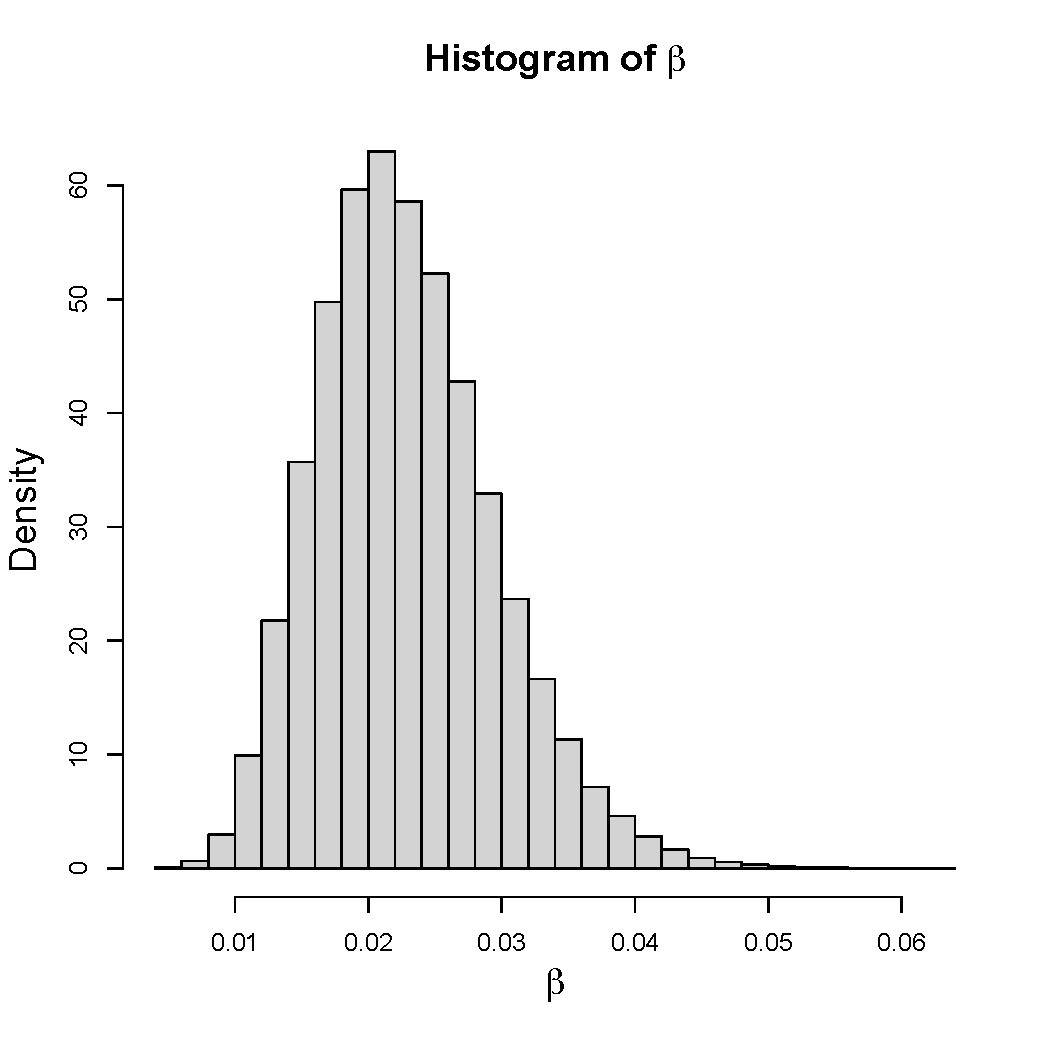
\includegraphics[width=3in]{bayes_figs/beta_hist.pdf}\quad
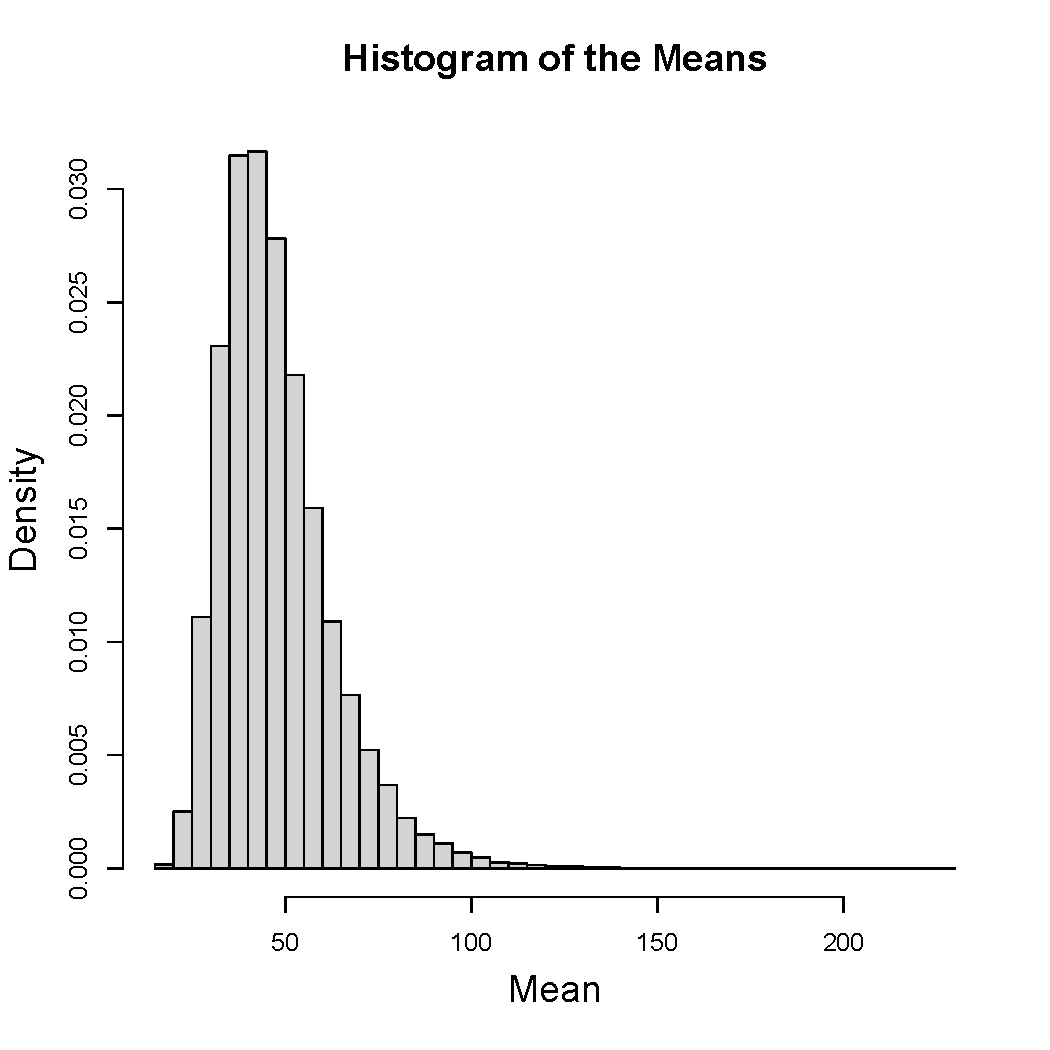
\includegraphics[width=3in]{bayes_figs/mean_hist.pdf}\quad
\end{figure}

Compare that credible interval with a $t$-interval and a bootstrapping interval: % sample size not big enough for t. Hard to justify that the entire population looks just like the sample for bootstrapping.

\begin{verbatim}
t.test(x)$conf.int
[1] 13.06527 74.36806
set.seed(2024)
means <- c()
for(i in 1:10000) {  
  index <- sample(1:length(x), length(x), replace = T)
  means[i] <- mean(x[index])
}
quantile(means, c(0.025, 0.975))
    2.5%    97.5% 
20.24979 72.30875 
\end{verbatim}
\phantom{.}\vspace{-.1in}
\begin{figure}[H] \hspace{0.2in} \begin{picture}(20,1)(0,0)
\put(-20,35){\framebox(130,28)}
\put(-22,161){\framebox(140,16)}
\end{picture} \end{figure}

\vspace{-0.4in}

\ub{Summary}:
\begin{itemize}
\item We assign a prior distribution to the parameter we are trying to estimate.
\item We assign a likelihood function to the data based on what we assume the population to look like or what distribution fits are data best.
\item We obtain a function that is proportional to the posterior for our parameter by multiplying the prior and likelihood together.
\item We identify what distribution has a kernel like the one we see in our posterior (thinking of our parameter now as $x_i$).
\item We obtain lots of samples from that posterior distribution.
\item We take the $\frac{\alpha}{2}th$ and $(1-\frac{\alpha}{2})th$ quantiles to obtain the $(1-\alpha)100\%$ credible intervals.
\begin{itemize}
\item That credible interval is the Bayesian version of a confidence interval and is used for inference on the parameter.
\end{itemize}
\end{itemize}

\newpage



\centerline{\fbox{\bf MCMC Sampling}}

MCMC stands for \uline{Markov chain Monte Carlo} and MCMC methods are a class of algorithms for sampling from a probability distribution. Monte Carlo sampling is the process of relying on many random samples to obtain numerical results and a \ub{Markov chain} is a process in which the next event depends only on the previous event. We will discuss two MCMC sampling methods: Gibbs sampling and Metropolis sampling. \\

\fbox{\bf Gibbs Sampling}

The \uline{basic Gibbs sampler} is used in much the same way as we saw on the previous few pages. We sample directly from a posterior distribution to obtain parameter values. With Gibbs sampling, however, we can sample from more than one distribution at a time while updating our parameter values as we go. The steps are shown below with two parameters, $\theta_1$ and $\theta_2$, but this can scale to any number of parameters.
\begin{enumerate}
\item Write down the posterior distributions for both $\theta_1$ and $\theta_2$: $p(\theta_1|\boldsymbol{x},\theta_2)$ and $p(\theta_2|\boldsymbol{x},\theta_1)$.
\item Select starting values for $\theta_1$ and $\theta_2$ called $\theta_1^{(0)}$ and $\theta_2^{(0)}$.
\item Generate, in turn,\\
\begin{align*}
\theta_1^{(i+1)}& \text{ from } p\left(\theta_1|\boldsymbol{x},\theta_2^{(i)}\right)\\
\theta_2^{(i+1)}& \text{ from } p\left(\theta_2|\boldsymbol{x},\theta_1^{(i+1)}\right)
\end{align*}
\item Increment $i$ and return to step 3. Continue until you obtain the number of desired samples.\\
\end{enumerate}

\underline{Example}: Assume a normal likelihood function with: $x_i|\mu,\sigma^2\sim N(\mu,\sigma^2)$. Let $\mu$ have a normal prior with $\mu\sim N(25,100)$ and let the precision $\tau=1/\sigma^2$ have a gamma prior with $\tau\sim \text{Gam}(5,1/2)$. Additionally, let $\boldsymbol{x}=(23.3, 14.5, 19.0, 20.2,  5.4, 23.8, 21.3, 12.8, 17.6, 19.8,$\\
$ 11.0, 21.5, 15.7, 22.1, 21.0, 13.7, 14.9, 13.8, 17.1, 11.3)$.

In this case, $n=20$, $\sigma^2_0=100$, $\mu_0=25$, $\alpha_0=5$, $\beta_0=1/2$, and $\overline{x}=16.99$.

\uline{Step 1}: Since these are conjugate priors, we have that\\
$\mu|\boldsymbol{x},\tau\sim N\left(\dfrac{1}{\frac{1}{\sigma^2_0}+\frac{n}{\sigma^2}}\left[\dfrac{\mu_0}{\sigma^2_0}+\dfrac{n\bar{x}}{\sigma^2}\right],\dfrac{1}{\frac{1}{\sigma^2_0}+\frac{n}{\sigma^2}}\right)=N\left(\dfrac{1}{\frac{1}{100}+20\tau}\left[\dfrac{25}{100}+339.8\tau\right],\dfrac{1}{\frac{1}{100}+20\tau}\right)$\\

and\\
$\tau|\boldsymbol{x},\mu\sim\text{Gam}\left(\alpha_0+n/2,\beta_0+\dfrac{\sum_{i=1}^n(x_i-\mu)^2}{2}\right)=\text{Gam}\left(15,\dfrac{1}{2}+\dfrac{\sum_{i=1}^n(x_i-\mu)^2}{2}\right)$\\ \\

\uline{Step 2}: The starting values usually do not matter too much. I will start each at the mean of their prior: $\mu^{(0)}=25$ and $\tau^{(0)}=10$.\\

\uline{Step 3}: Generate each of the following:
$$
\mu^{(i+1)} \text{ from } N\left(\dfrac{1}{\frac{1}{100}+20\tau^{(i)}}\left[\dfrac{25}{100}+339.8\tau^{(i)}\right],\dfrac{1}{\frac{1}{100}+20\tau^{(i)}}\right)
$$
$$
\tau^{(i+1)} \text{ from } \text{Gam}\left(15,\dfrac{1}{2}+\dfrac{\sum_{i=1}^n(x_i-\mu^{(i+1)})^2}{2}\right)
$$

\vspace{-.1in}

\uline{Step 4}: Repeat for 10,000 samples.

The {\bf R} code is shown below:
\begin{verbatim}
x <- c(23.3, 14.5, 19.0, 20.2,  5.4, 23.8, 21.3, 12.8, 17.6, 19.8,
   11.0, 21.5, 15.7, 22.1, 21.0, 13.7, 14.9, 13.8, 17.1, 11.3)
nsamps <- 10000
mu <- rep(0, nsamps)  # Initialize the mu vector
mu[1] <- 25           # Starting value of mu
tau <- rep(0, nsamps) # Initialize the tau vector
tau[1] <- 10          # Starting value of tau
for(i in 1:(nsamps - 1)) {
     mu[i+1] <- rnorm(n = 1, mean = 1/(1/100 + 20*tau[i]) * (25/100 + 339.8*tau[i]),
                      sd = 1/(1/100 + 20*tau[i]))
     tau[i+1] = rgamma(n = 1, shape = 15, rate = 1/2 + 1/2 * sum((x - mu[i+1])^2))
}
\end{verbatim}

\vspace{-.2in}

\begin{figure}[H]
\centering
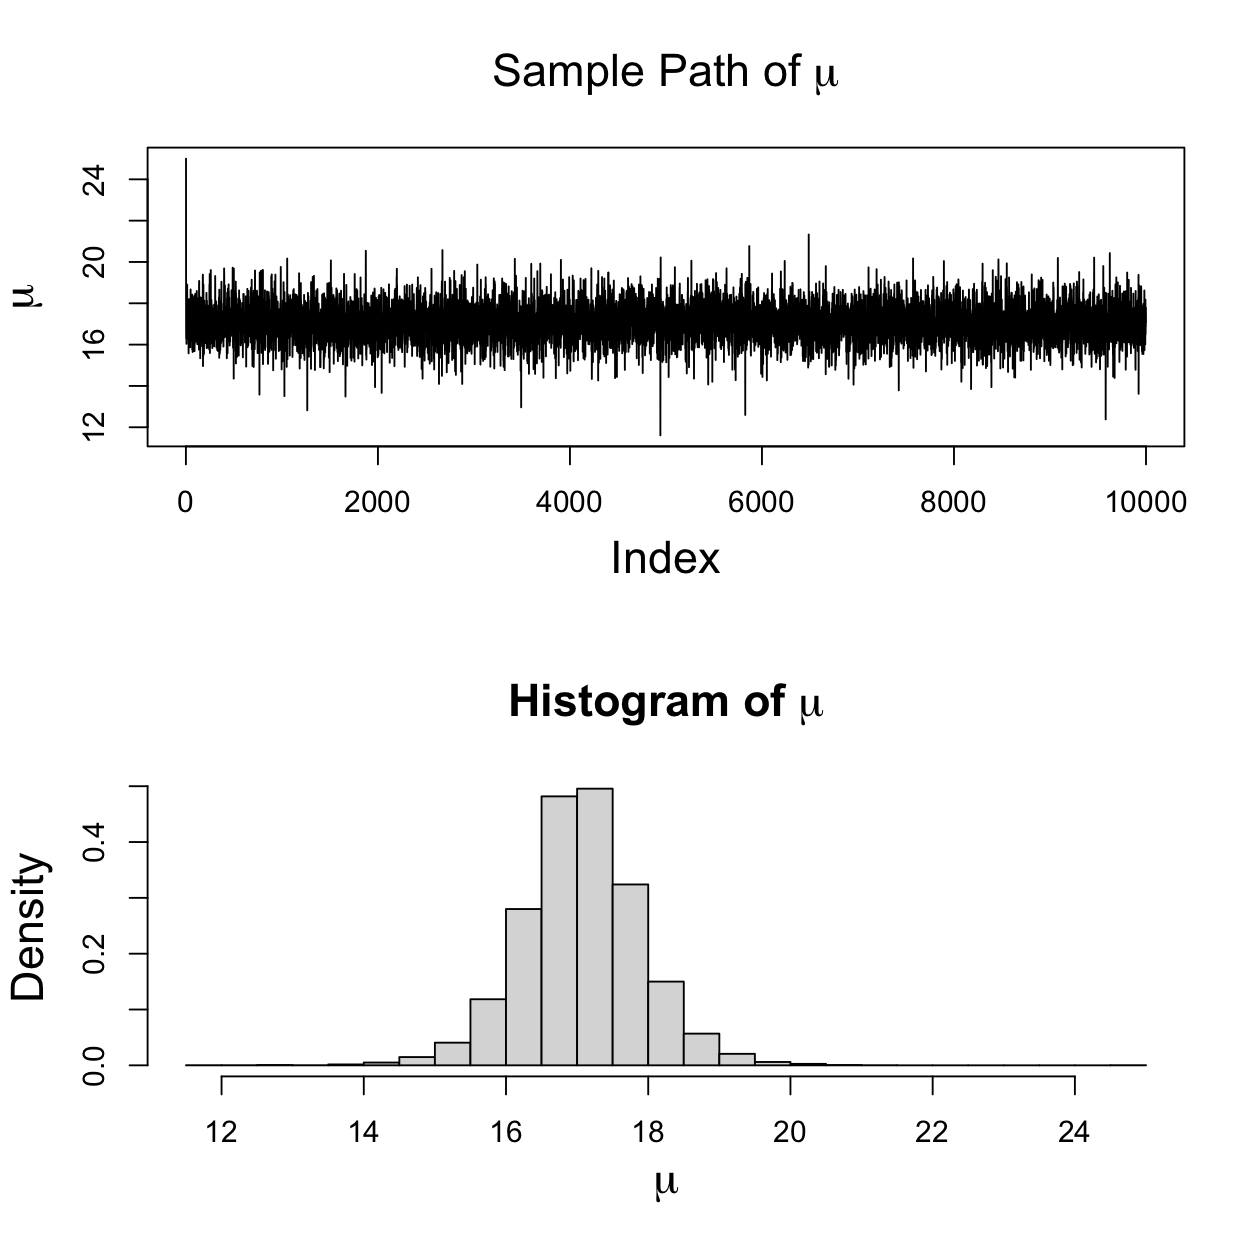
\includegraphics[width=3.1in,height=2.4in]{bayes_figs/Plots_mu.png} % 15.36708 18.75692
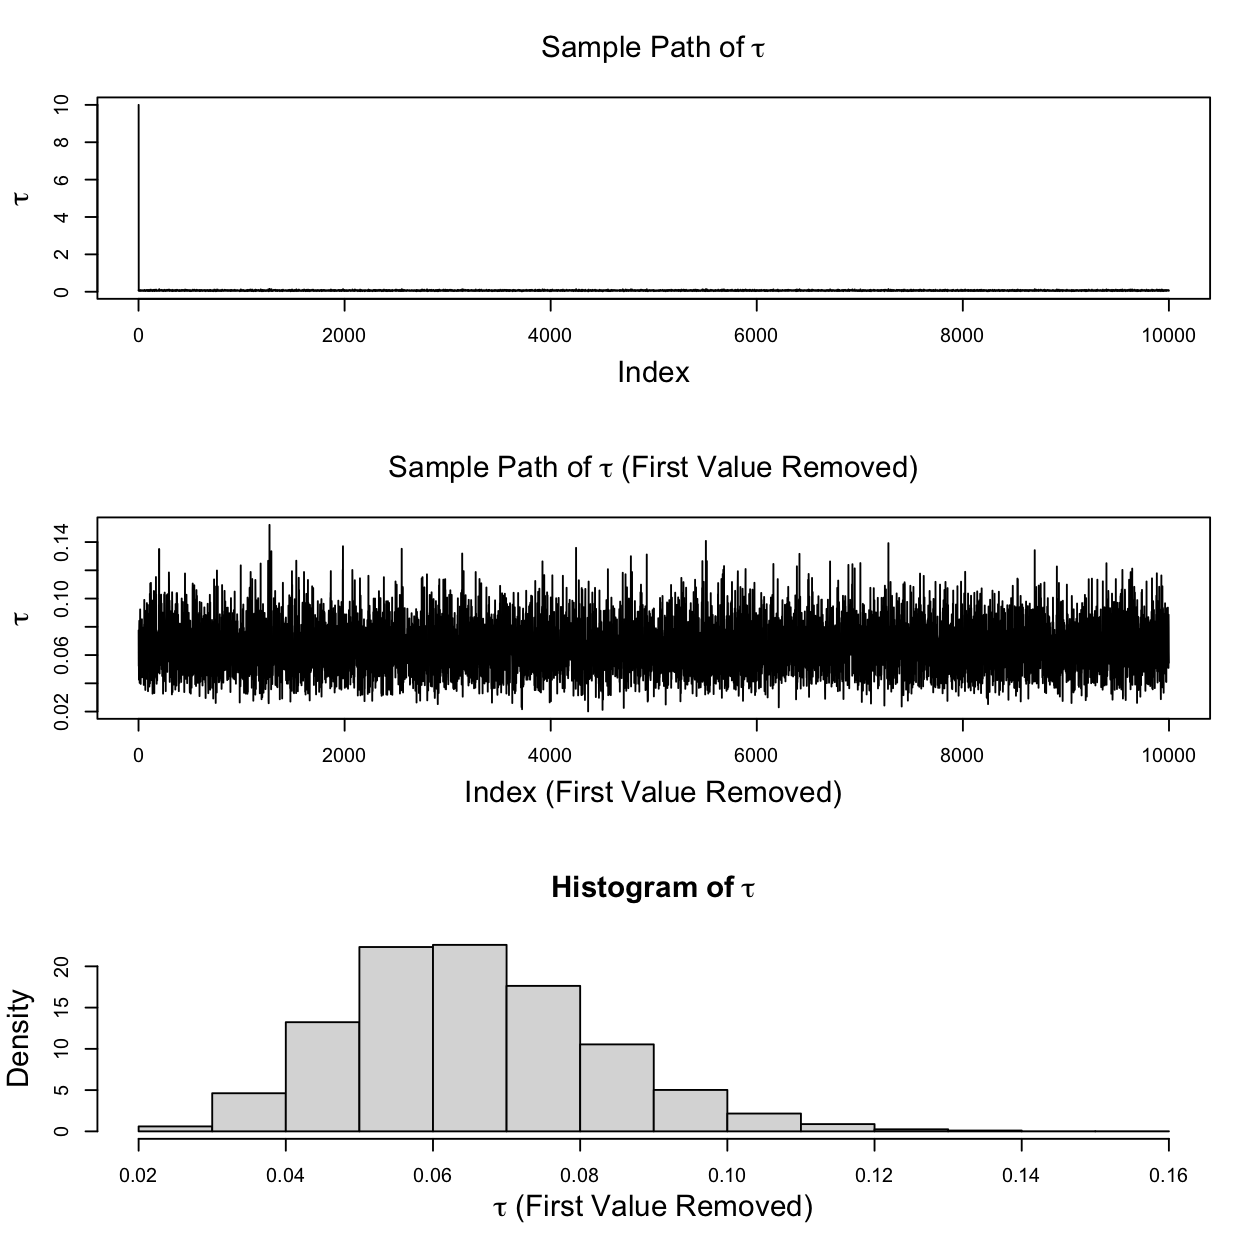
\includegraphics[width=3.1in,height=2.4in]{bayes_figs/Plots_tau.png} % 0.03577438 0.10296530
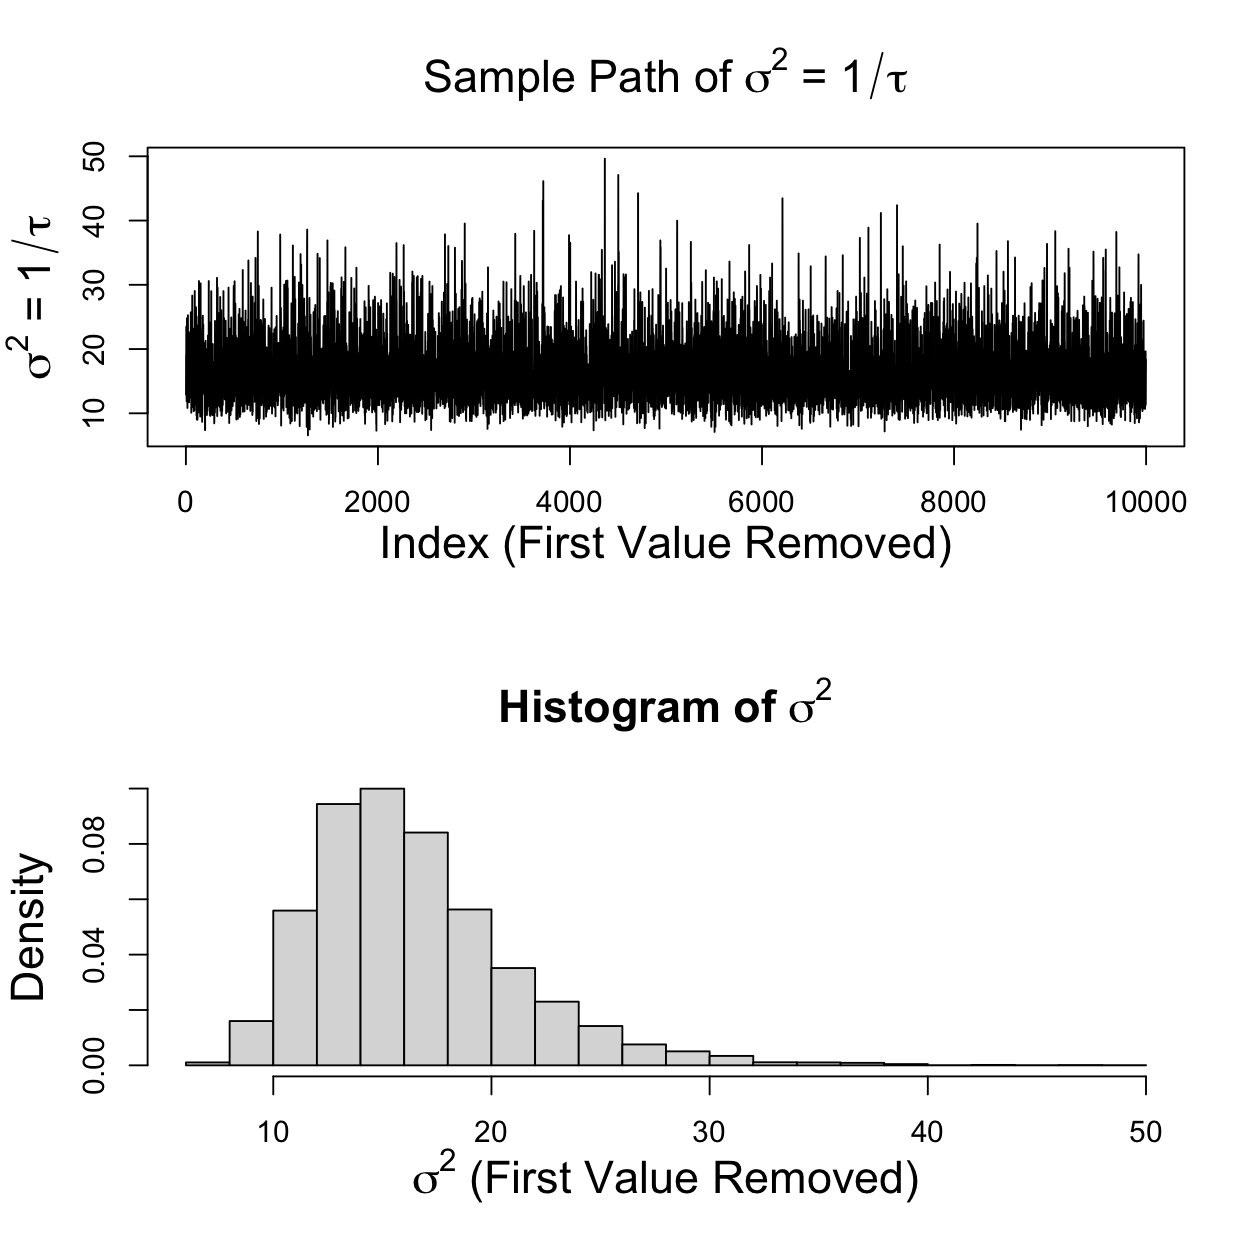
\includegraphics[width=3.1in,height=2.4in]{bayes_figs/Plots_sigma.png} % 9.712009 27.952968
\end{figure}

\fbox{\bf Metropolis Sampling}

The Gibbs sampler is the go-to option when we can write down exactly what distribution we will sample from. Having conjugate priors makes this simpler, but in other cases it still may be possible to figure out exactly what distribution the parameter will follow. 

However, it is often the case that no conjugate prior will exist and the distribution the parameter follows is not a known one. If, however, we can write down the distribution up to a proportionality constant, we can still obtain samples from the unknown distribution using the Metropolis sampling method. The steps for this method are given here: 
\begin{enumerate}
\item Write down $f(\theta|\boldsymbol{x})$ that is proportional to the posterior $p(\theta|\boldsymbol{x})$.
\item Choose a symmetric proposal distribution distribution $g(\theta)$ that is used to obtain candidates of $\theta$ that will either be accepted or rejected as a new sample value. Using a normal distribution works well.
\item Select the starting value of $\theta$ called $\theta^{(0)}$.
\item For each iteration $i$, do the following:
\begin{enumerate}
\item Generate a candidate for $\theta^{(i+1)}$ called $\theta^*$ from the proposal distribution $g(\theta^*|\theta^{(i)})$.
\item Calculate an acceptance ratio $R=f(\theta^*|\boldsymbol{x})/f(\theta^{(i)}|\boldsymbol{x})$.
\item Generate a uniform random number $u$ between 0 and 1.
\begin{enumerate}
\item[(1)] If $u\le R$, accept the candidate and let $\theta^{(i+1)}=\theta^*$.
\item[(2)] If $u>R$, reject the candidate and let $\theta^{(i+1)}=\theta^{(i)}$.
\end{enumerate}
\end{enumerate}
\item Increment $i$ and return to step 4. Continue until you obtain the number of desired samples.\\
\end{enumerate}

Note that step 4 (c) can be numerically unstable, so it is often the case that we will accept the candidate if $\log(u)\le \log\left(f(\theta^*|\boldsymbol{x})\right)-\log\left(f(\theta^{(i)}|\boldsymbol{x})\right)$ instead.\\

\underline{Example}: Let's use the grocery data from Notes 11\\
again and obtain samples from the posterior\\
distribution of the standard deviation, $\sigma$. According\\
to figures form 2019 surveys out of the Bureau of\\
Labor Statistics, the average cost of groceries per\\
year is \$4,643 per household. Assuming a shopping\\
trip 60 times per year, that will give us a true average\\
amount spent of \$77 per trip. So, we will assume $\mu=77$. 

Looking at the histogram of our data, we can see it is\\
clearly not normal. Fitting a distribution to it, the gamma\\
distribution works fairly well. In the plot shown here, $\alpha=0.8569$ and $\beta=0.0163$, but we will use MCMC to obtain estimates for those. 
\vspace{-2.9in}

\begin{figure}[H]
\raggedleft
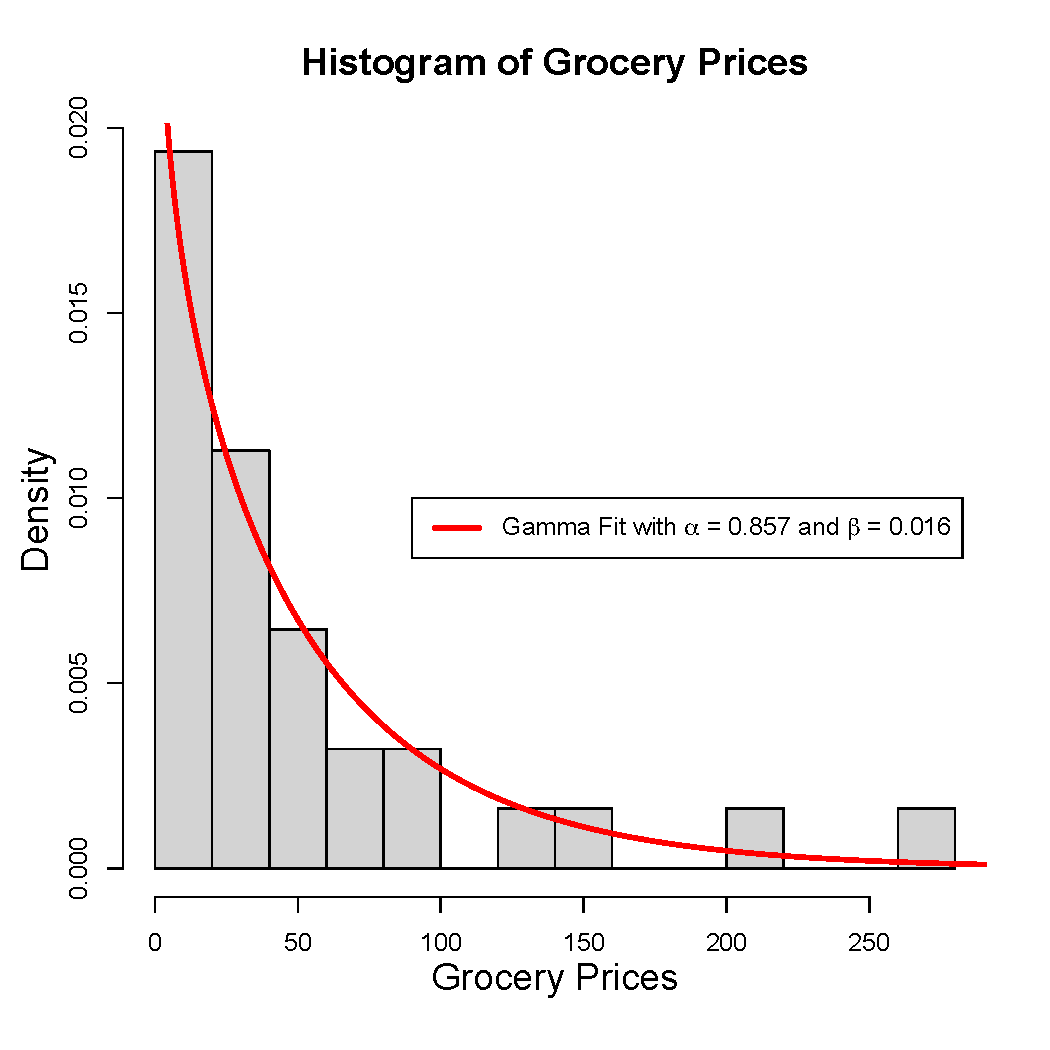
\includegraphics[width=2.5in]{bayes_figs/Grocery_hist.pdf}
\end{figure}

\newpage

\uline{Step 1}: Write down $f(\theta|\boldsymbol{x})$ that is proportional to the posterior $p(\theta|\boldsymbol{x})$.\\
Begin with $p(x_i|\alpha,\beta)=\dfrac{\beta^\alpha}{\Gamma(\alpha)}x_i^{\alpha-1}e^{-\beta x_i}$. Now, let's reparametrize so we have this distribution in terms of $\mu$ and $\sigma^2$. We know $\mu=\alpha/\beta$ and $\sigma^2=\alpha/\beta^2$. Solving these for $\alpha$ and $\beta$ give us:
\vspace{1in}

So $\alpha=\mu^2/\sigma^2$ and $\beta=\mu/\sigma^2$. Therefore, 
$p(x_i|\mu,\sigma)=\dfrac{(\mu/\sigma^2)^{\mu^2/\sigma^2}}{\Gamma(\mu^2/\sigma^2)}x_i^{\mu^2/\sigma^2-1}e^{-\mu x_i/\sigma^2}$

So $p(\boldsymbol{x}|\mu,\sigma)=$

\vspace{1.5in}

Now, for the prior of $\sigma$, an exponential distribution makes sense since $\sigma$ cannot be negative. Let's chose a rate parameter fairly small so the variance is large. That will lead to the prior being less restricting. Let $\sigma\sim \text{Exp}(1/50)$ so $p(\sigma)=\dfrac{1}{50}e^{-\sigma/50}$. Therefore, the posterior is 
\begin{align*}
p(\sigma|\boldsymbol{x},\mu)&\propto  \dfrac{1}{50}e^{-\sigma/50}\left(\dfrac{(\mu/\sigma^2)^{\mu^2/\sigma^2}}{\Gamma(\mu^2/\sigma^2)}\right)^n\prod_{i=1}^nx_i^{\mu^2/\sigma^2-1}\exp\left\{-\mu/\sigma^2\sum_{i=1}^nx_i\right\}\\
&\propto\dfrac{(\mu/\sigma^2)^{n\mu^2/\sigma^2}}{\Gamma(\mu^2/\sigma^2)^n}\prod_{i=1}^nx_i^{\mu^2/\sigma^2-1}\exp\left\{-\sigma/50-\mu/\sigma^2\sum_{i=1}^nx_i\right\}= f(\sigma|\boldsymbol{x},\mu)
\end{align*}
This is certainly not a nice looking or known distribution for $\sigma$ and we only know it up to a proportionality constant. We can still sample from this using the Metropolis algorithm, though!

When we do the metropolis algorithm, it will be useful to use $\log(f(\sigma|\boldsymbol{x},\mu))$ since $f(\sigma|\boldsymbol{x},\mu)$ will often be numerically unstable:
\begin{align*}
\log\left(f(\sigma|\boldsymbol{x},\mu)\right)&=\log\left(\dfrac{(\mu/\sigma^2)^{n\mu^2/\sigma^2}}{\Gamma(\mu^2/\sigma^2)^n}\prod_{i=1}^nx_i^{\mu^2/\sigma^2-1}\exp\left\{-\sigma/50-\mu/\sigma^2\sum_{i=1}^nx_i\right\}\right)\\
&=\frac{n\mu^2}{\sigma^2}\log(\mu/\sigma^2)-n\log\left(\Gamma(\mu^2/\sigma^2)\right)+(\mu^2/\sigma^2-1)\sum_{i=1}^n\log(x_i)-\frac{\sigma}{50}-\frac{\mu}{\sigma^2}\sum_{i=1}^nx_i
%&=n\mu/\sigma^2\log\left(\mu/\sigma^2\right)-n\log\left(\Gamma(\mu^2/\sigma^2)\right)+(\mu^2/\sigma^2-\mu/\sigma^2-1)\sum_{i=1}^nx_i-\sigma/5
\end{align*}

\newpage

\uline{Step 2}: Choose the proposal distribution. We will let the proposal distribution be normal.\newline

\vspace{-.2in}

\uline{Step 3}: Select the starting value of $\sigma$. Let's begin at $\sigma^{(0)}=s=64$. 

\uline{Step 4}: Generate next sample:
\begin{enumerate}
\item[(a)] Generate a random value from the proposal. The first time through, $i=0$. We will use the previous value of $\sigma$, $\sigma^{(i)}$ as the mean of the proposal with a standard deviation of 10. The value of 10 can be changed if it doesn't work well. $\sigma^*\sim N(\sigma^{(i)},10)$. Suppose doing this gives $\sigma^*= 70$.
\item[(b)]  Calculate an acceptance ratio  $R=f(\sigma^*|\boldsymbol{x},\mu)/f(\sigma^{(i)}|\boldsymbol{x},\mu)$ or find $\log(R)=\log(f(\sigma^*|\boldsymbol{x},\mu))-\log(f(\sigma^{(i)}|\boldsymbol{x},\mu)).$

In our case, since we are saying $\mu=77$, and $n=31$, we have:
\begin{align*}
f(\sigma^*|\boldsymbol{x},\mu)&=\dfrac{(77/(\sigma^*)^2)^{31\cdot 77^2/(\sigma^*)^2}}{\Gamma(77^2/(\sigma^*)^2)^{31}}\prod_{i=1}^{31}x_i^{77^2/(\sigma^*)^2-1}\exp\left\{-\sigma^*/50-77/(\sigma^*)^2\sum_{i=1}^{31}x_i\right\}\\
&=\dfrac{(77/70^2)^{31\cdot 77^2/70^2}}{\Gamma(77^2/70^2)^{31}}\prod_{i=1}^{31}x_i^{77^2/70^2-1}\exp\left\{-70/50-77/70^2\sum_{i=1}^{31}x_i\right\}\\
&=1.21888\times 10^{-69} \text{ (crazy small number)}\\
f(\sigma^{(i)}|\boldsymbol{x},\mu)&=\dfrac{(77/(\sigma^{(i)})^2)^{31\cdot 77^2/(\sigma^{(i)})^2}}{\Gamma(77^2/(\sigma^{(i)})^2)^{31}}\prod_{i=1}^{31}x_i^{77^2/(\sigma^{(i)})^2-1}\exp\left\{-\sigma^{(i)}/50-77/(\sigma^{(i)})^2\sum_{i=1}^{31}x_i\right\}\\
&=\dfrac{(77/64^2)^{31\cdot 77^2/64^2}}{\Gamma(77^2/64^2)^{31}}\prod_{i=1}^{31}x_i^{77^2/64^2-1}\exp\left\{-64/50-77/64^2\sum_{i=1}^{31}x_i\right\}\\
&=1.219423\times10^{-70} \text{ (slightly crazier small number)}\\
R&=f(\sigma^*|\boldsymbol{x},\mu)/f(\sigma^{(i)}|\boldsymbol{x},\mu)=9.995544
\end{align*}
Using the $\ell(\sigma)=\log\left(f(\sigma|\boldsymbol{x},\mu)\right)$ instead gives us 
\begin{align*}
\ell(\sigma^*)&=31\cdot77^2/(\sigma^*)^2\log(77/(\sigma^*)^2)-31\log\left(\Gamma(77^2/(\sigma^*)^2)\right)\\
&\hspace{.5in}+(77^2/(\sigma^*)^2-1)\sum_{i=1}^n\log(x_i)-(\sigma^*)/50-77/(\sigma^*)^2\sum_{i=1}^nx_i\\
&=31\cdot77^2/70^2\log(77/70^2)-31\log\left(\Gamma(77^2/70^2)\right)\\
&\hspace{.5in}+(77^2/70^2-1)\sum_{i=1}^n\log(x_i)-70/50-77/70^2\sum_{i=1}^nx_i\\
&=-158.6804\\
\ell(\sigma^{(i)})&=31\cdot77^2/64^2\log(77/64^2)-31\log\left(\Gamma(77^2/64^2)\right)\\
&\hspace{.5in}+(77^2/64^2-1)\sum_{i=1}^n\log(x_i)-64/50-77/64^2\sum_{i=1}^nx_i\\
&=-160.9826
\end{align*}

\item[(c)] Now generate a random number between 0 and 1. {\bf R} can do this with the \texttt{runif(1)} command. Doing this gave me $u=0.4061828$. Since $u<R=9.995544$ \\(or $\log(u)=-0.900952<\ell(\sigma^*)-\ell\left(\sigma^{(i)}\right)=2.3022)$, we accept the candidate as the new sample as $\sigma^{(i+1)}=\sigma^{(1)}=\sigma^{*}=70$.
\end{enumerate}

\uline{Step 5}: Repeat this process thousands of times.
\begin{figure}[H]
\centering
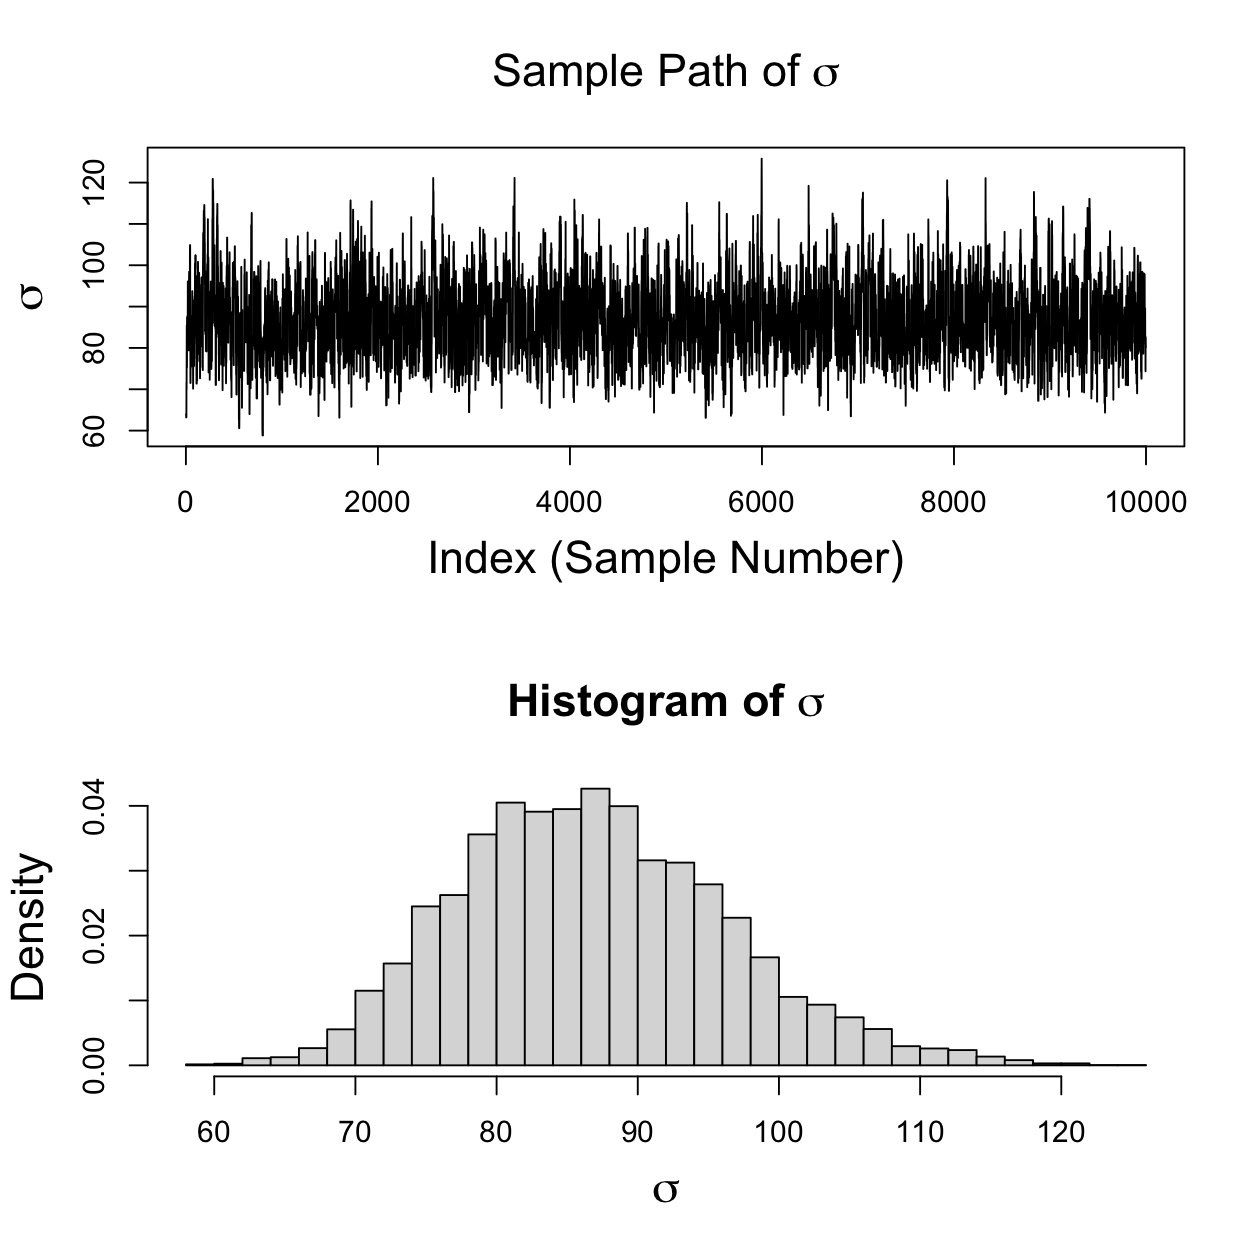
\includegraphics[width=4.7in,height=3.1in]{bayes_figs/Plots_sigma_metropolis.png} 
\end{figure}
\vspace{-.3in}
\begin{verbatim}
grocery <- c(1,3,4,5,5,8,11,12,15,15,16,19,21,25,26,27,30,35,35,46,50,
      55,57,72,78,85,93,137,158,212,269)
nsamps <- 10000
sigma <- rep(0,nsamps)
sigma[1] <- 64
mu <- 77
n <- length(grocery) # 31
for(i in 1:(nsamps - 1)) {
    sigma_star <- rnorm(1, sigma[i], 10)
    logf1 <- n * mu^2 / sigma_star^2 * log(mu / sigma_star^2) -
            n * log(gamma(mu^2 / sigma_star^2)) +
            (mu^2 / sigma_star^2 - 1) * sum(log(grocery)) -
            sigma_star / 50 - mu / sigma_star^2 * sum(grocery)
    logf2 <- n * mu^2 / sigma[i]^2 * log(mu/sigma[i]^2) -
            n * log(gamma(mu^2 / sigma[i]^2)) +
            (mu^2 / sigma[i]^2 - 1) * sum(log(grocery)) -
            sigma[i] / 50 - mu / sigma[i]^2 * sum(grocery)
    if(log(runif(1)) < (logf1 - logf2)) {
     	sigma[i+1] <- sigma_star
    } else {
     	sigma[i+1] <- sigma[i]
    }
}
\end{verbatim}

\newpage

\fbox{\bf MCMC Diagnostics}

There are two important diagnostics we will look at when doing MCMC sampling. Both of which have to do with how well the sampling chains mix. 
\begin{enumerate}
\item Plots of the sampling chain.
\item The integrated autocorrelation time and effective sample size.
\end{enumerate}

\ub{Plots of the sampling chain(s)}

The primary diagnostic tool for evaluating\\
MCMC sampling is observing the sampling\\
chains. Ideally, each sample in the chain will\\
be independent from all others. Since the\\
posterior distributions rely on the previous\\
iteration, that is not going to be the case, but\\
we would like to minimize the number of\\
previous iterations on which the current one\\
depends. A good-looking sampling chain is one\\
that essentially looks like noise, with no\\
discernible patterns or paths. 
\vspace{-2.4in}
\begin{figure}[H]
\raggedleft
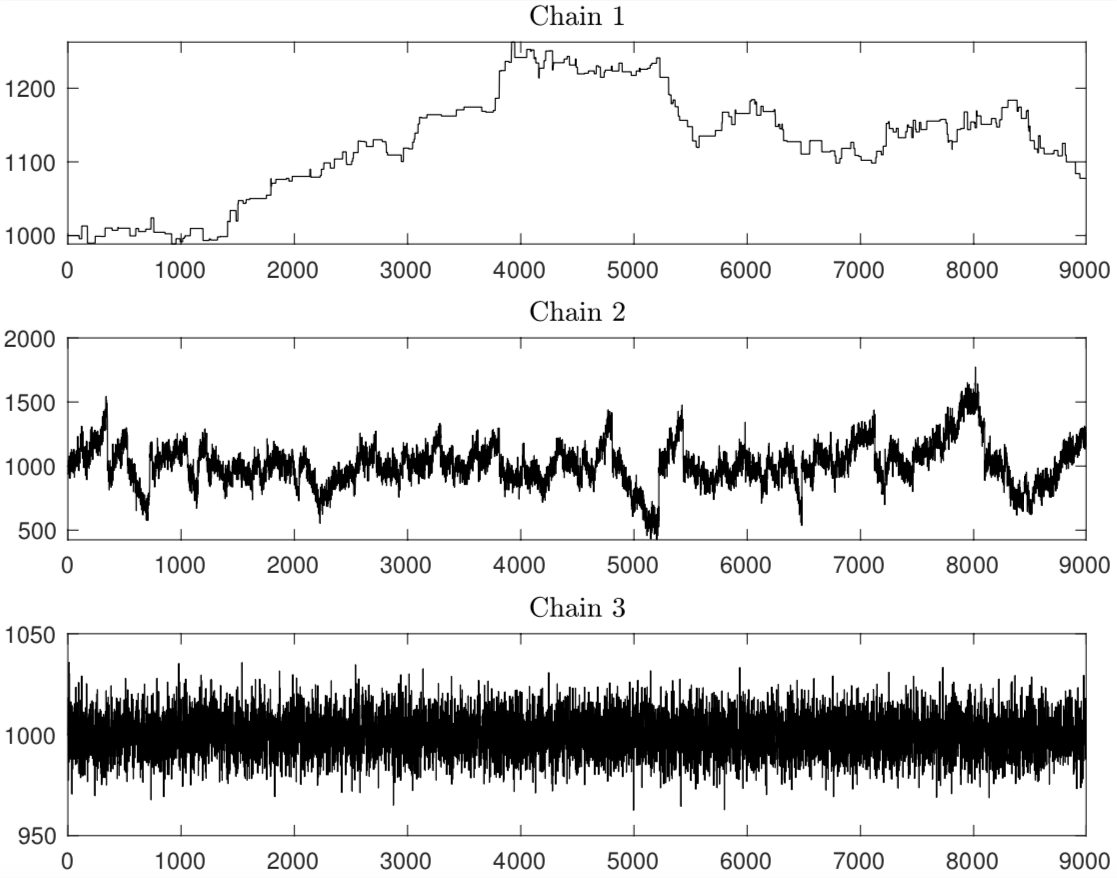
\includegraphics[width=3in]{bayes_figs/chain_example.png}
\end{figure}

\vfill

\ub{Integrated Autocorrelation Time and Effective Sample Size}

To check how correlated the chain is with itself, we can calculate the \uline{integrated autocorrelation time} of the chain. We can do this by taking
$
\ds\hat{\tau}_{\text{int}}=1+2\sum_{k=1}^\infty\hat{\rho}(k)
$
where $\hat{\rho}(k)$ is the correlation of the chain at a lag of $k$. For example, the autocorrelation of the chain on the previous page is given here. The \texttt{acf} function in {\bf R} can calculate the autocorrelation and make this plot.

\vspace{-.4in}
\begin{figure}[H]
\raggedleft
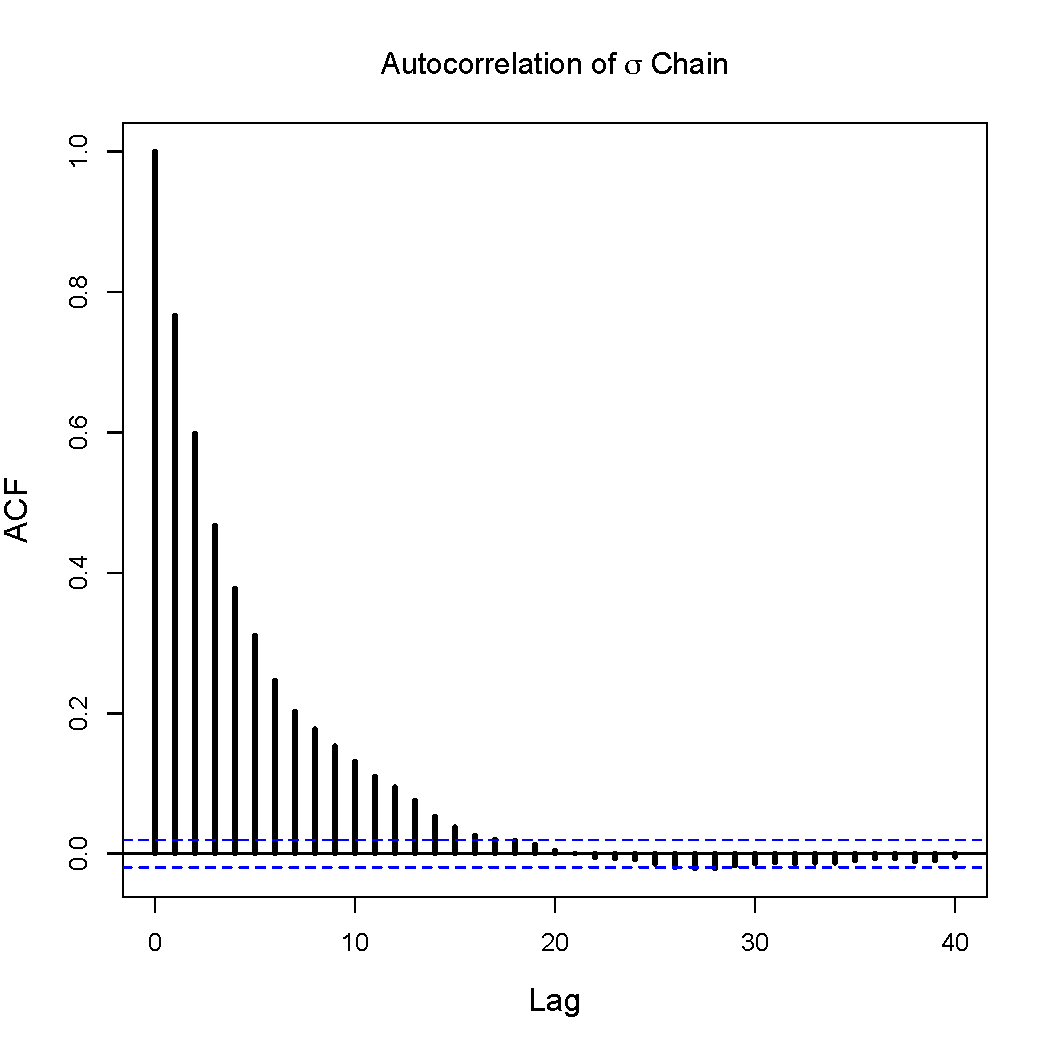
\includegraphics[width=3in]{bayes_figs/ACF.pdf} 
\end{figure}

\vspace{-1.5in}
Once we have $\hat{\tau}_{\text{int}}$, we can calculate the\\
\ub{effective sample size} as $K_{\text{ESS}}=K/\hat{\tau}_{\text{int}}$\\
where $K$ is the number of MCMC samples\\
in the chain.

In our example, $\hat{\tau}_{\text{int}}\approx 13$, so our essential sample\\
size is  $K_{\text{ESS}}=10000/13=769$. In order to get the\\
equivalent of 10,000 samples, we need to set the number of MCMC samples to 130,000.

\newpage

\uline{Back to grocery example}. What happens if the SD of the proposal distribution is changed?
\vspace{-.1in}
\begin{figure}[H]
\centering
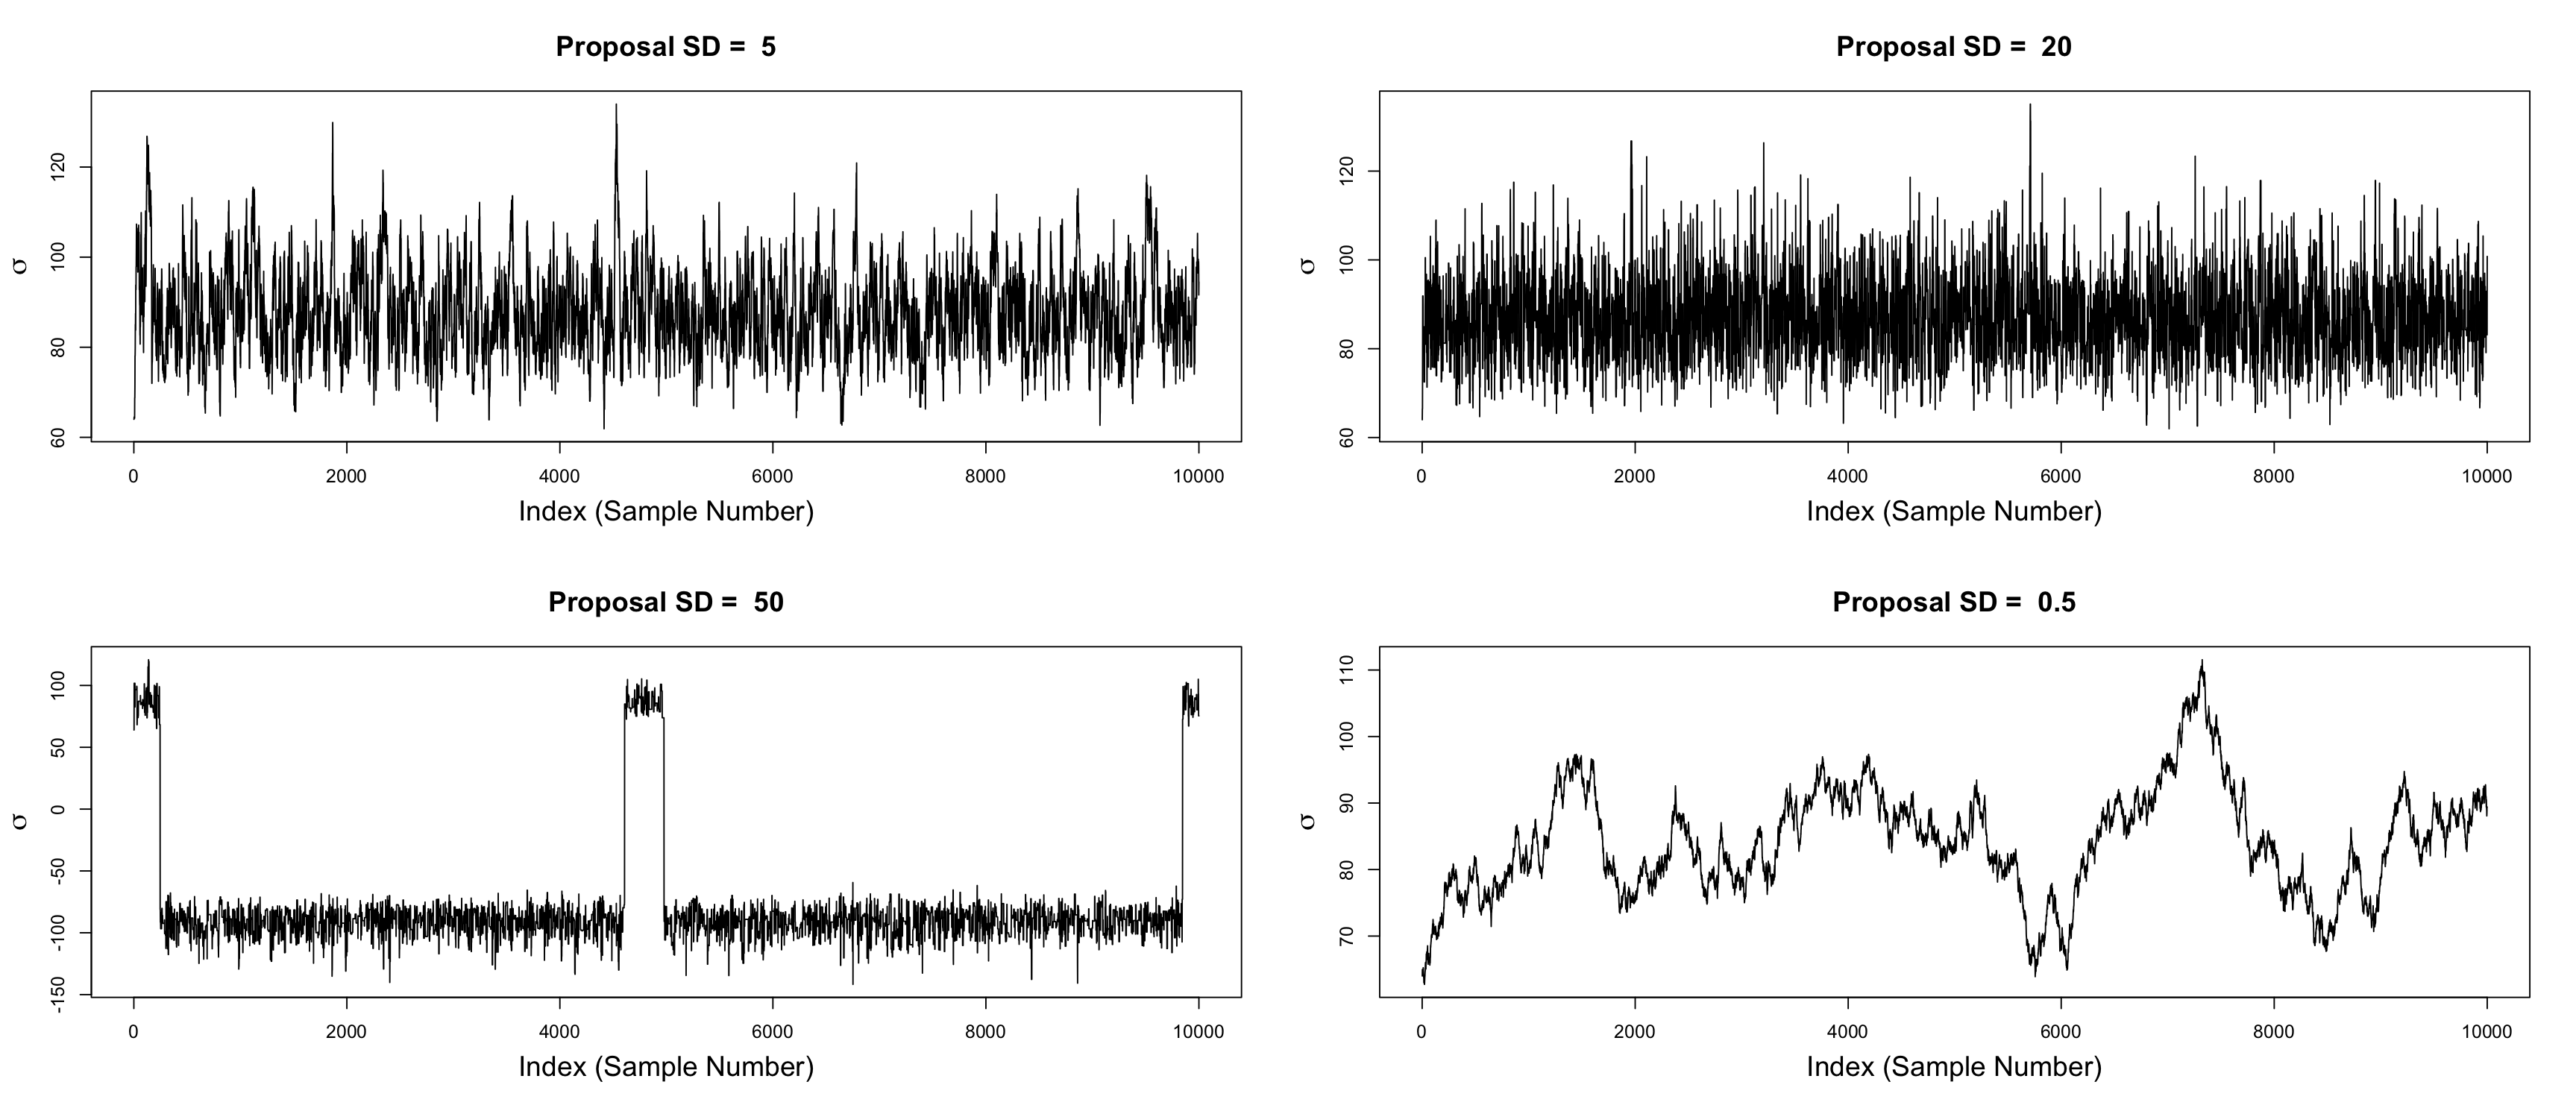
\includegraphics[width=6in,height=3.8in]{bayes_figs/Plots_differentSDs.png} 
\end{figure}
%\sigma_0 = 10, 20, 50, 2

\vspace{.2in}

What happens if the value we use for $\mu$ is changed? 
\vspace{.1in}
%  mu = 77: 71.1275 107.4342 
% mu = 100:  96.9501 145.1599 
% mu = 50: 44.75457 68.37335 
% mu = 29.56720 45.48971 
% based on the sample, we know the standard deviation should be similar (a bit larger) than the  mean
\begin{figure}[H]
\centering
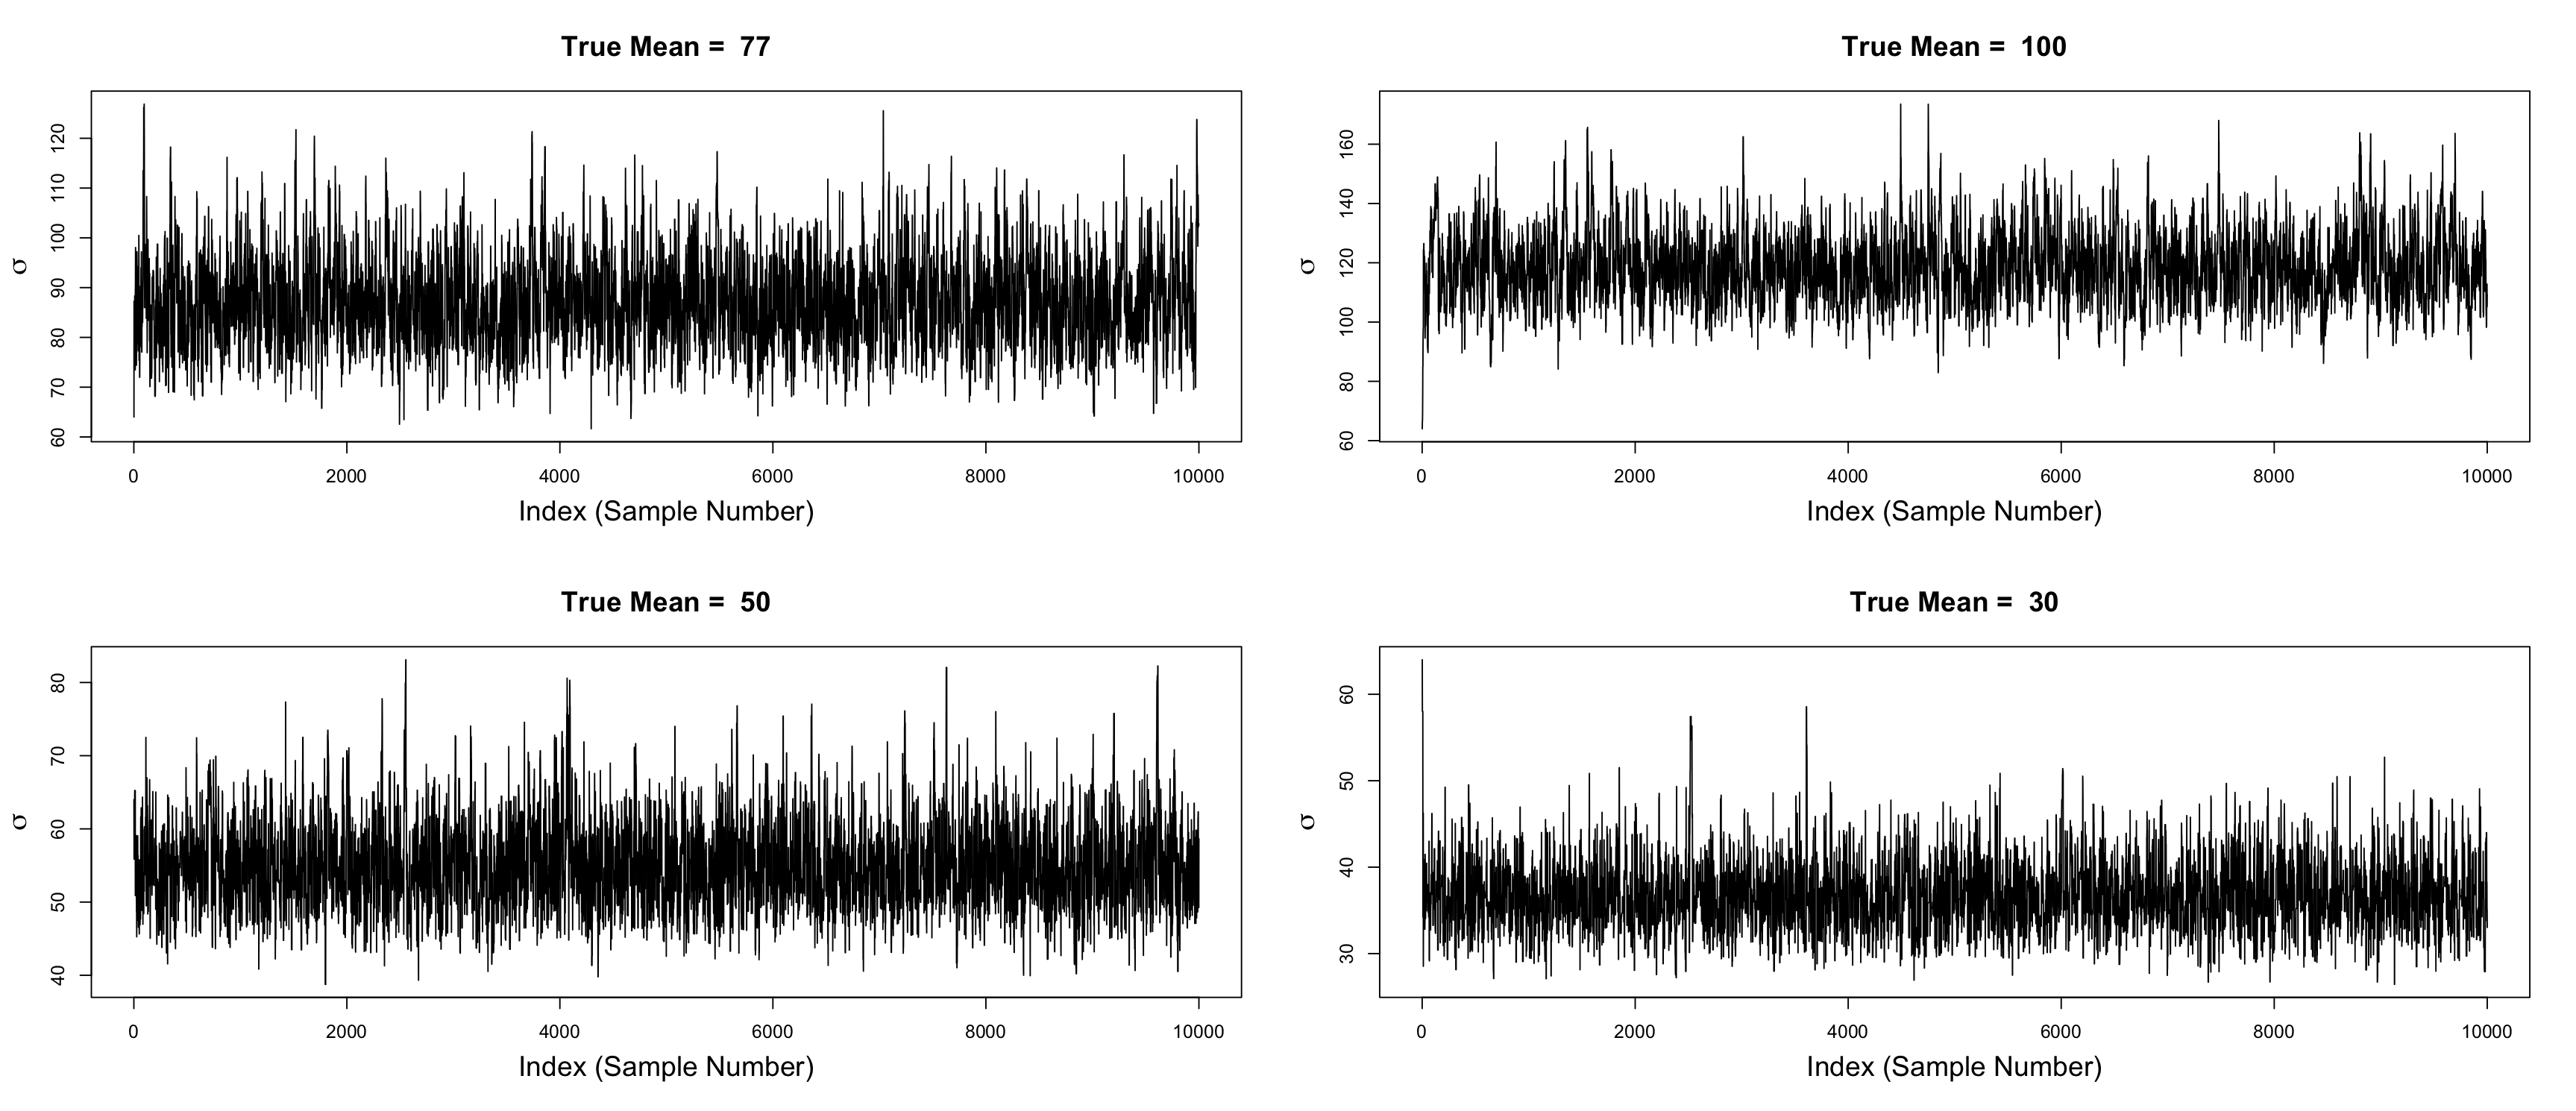
\includegraphics[width=6in,height=3.8in]{bayes_figs/Plots_differentmeans.png} 
\end{figure}

\newpage

\fbox{\bf Metropolis Sampling of Two Parameters}

Clearly, the value of $\mu$ influences the sample values of $\sigma$ a lot here. Instead of fixing $\mu$, we can sample values of $\mu$ and $\sigma$ simultaneously. Let's put a prior on $\mu$ of $\text{Exp}(1/70)$ so the mean is $70$ with a large variance. Then find the posterior for both $\mu$ and $\sigma$. Compare this to the posterior at the bottom of page 193:
\begin{align*}
p(\mu,\sigma|\boldsymbol{x})&\propto    \dfrac{1}{70}e^{-\mu/50}\dfrac{1}{50}e^{-\sigma/50}\left(\dfrac{(\mu/\sigma^2)^{\mu^2/\sigma^2}}{\Gamma(\mu^2/\sigma^2)}\right)^n\prod_{i=1}^nx_i^{\mu^2/\sigma^2-1}\exp\left\{-\mu/\sigma^2\sum_{i=1}^nx_i\right\}\\
&\propto\dfrac{(\mu/\sigma^2)^{n\mu^2/\sigma^2}}{\Gamma(\mu^2/\sigma^2)^n}\prod_{i=1}^nx_i^{\mu^2/\sigma^2-1}\exp\left\{-\mu/70-\sigma/50-\mu/\sigma^2\sum_{i=1}^nx_i\right\}= f(\mu,\sigma|\boldsymbol{x})
\end{align*}
So then 
\begin{align*}
\log\left(f(\mu,\sigma|\boldsymbol{x})\right)=\frac{n\mu^2}{\sigma^2}\log(\mu/\sigma^2)-n\log\left(\Gamma(\mu^2/\sigma^2)\right)+(\mu^2/\sigma^2-1)\sum_{i=1}^n\log(x_i)-\frac{\mu}{70}-\frac{\sigma}{50}-\frac{\mu}{\sigma^2}\sum_{i=1}^nx_i
\end{align*}
Then we can generate a candidate for both $\mu$ and $\sigma$ called $\mu^*$ and $\sigma^*$ and compare them to the previous values of $\mu$ and $\sigma$: $(\mu^{(i)},\sigma^{(i)})$.
\begin{verbatim}
nsamps <- 30000
sigma <- rep(0,nsamps)
sigma[1] <- 64
mu <- rep(0,nsamps)
mu[1] <- 77
n <- length(grocery) # 31
for(i in 1:(nsamps - 1)){
    mu_star <- rnorm(1, mu[i], 10)
    sigma_star <- rnorm(1, sigma[i], 10)
    logf1 <- n * mu_star^2 / sigma_star^2 * log(mu_star/sigma_star^2) -
	            n * log(gamma(mu_star^2 / sigma_star^2)) +
	            (mu_star^2 / sigma_star^2 - 1) * sum(log(grocery)) -
	            mu_star / 70 - sigma_star / 50 - mu_star / sigma_star^2 * sum(grocery)
    logf2 <- n * mu[i]^2 / sigma[i]^2 * log(mu[i] / sigma[i]^2) -
	            n * log(gamma(mu[i]^2 / sigma[i]^2)) +
	            (mu[i]^2 / sigma[i]^2 - 1) * sum(log(grocery)) -
	            mu[i] / 70 - sigma[i] / 50 - mu[i] / sigma[i]^2 * sum(grocery)
    if(log(runif(1)) < (logf1 - logf2)) {
		       mu[i+1] <- mu_star
	    	  sigma[i+1] <- sigma_star
	    } else {
	       mu[i+1] <- mu[i]
	       sigma[i+1] <- sigma[i]
	    }
}


\end{verbatim}

\newpage
\begin{figure}[H]
\centering
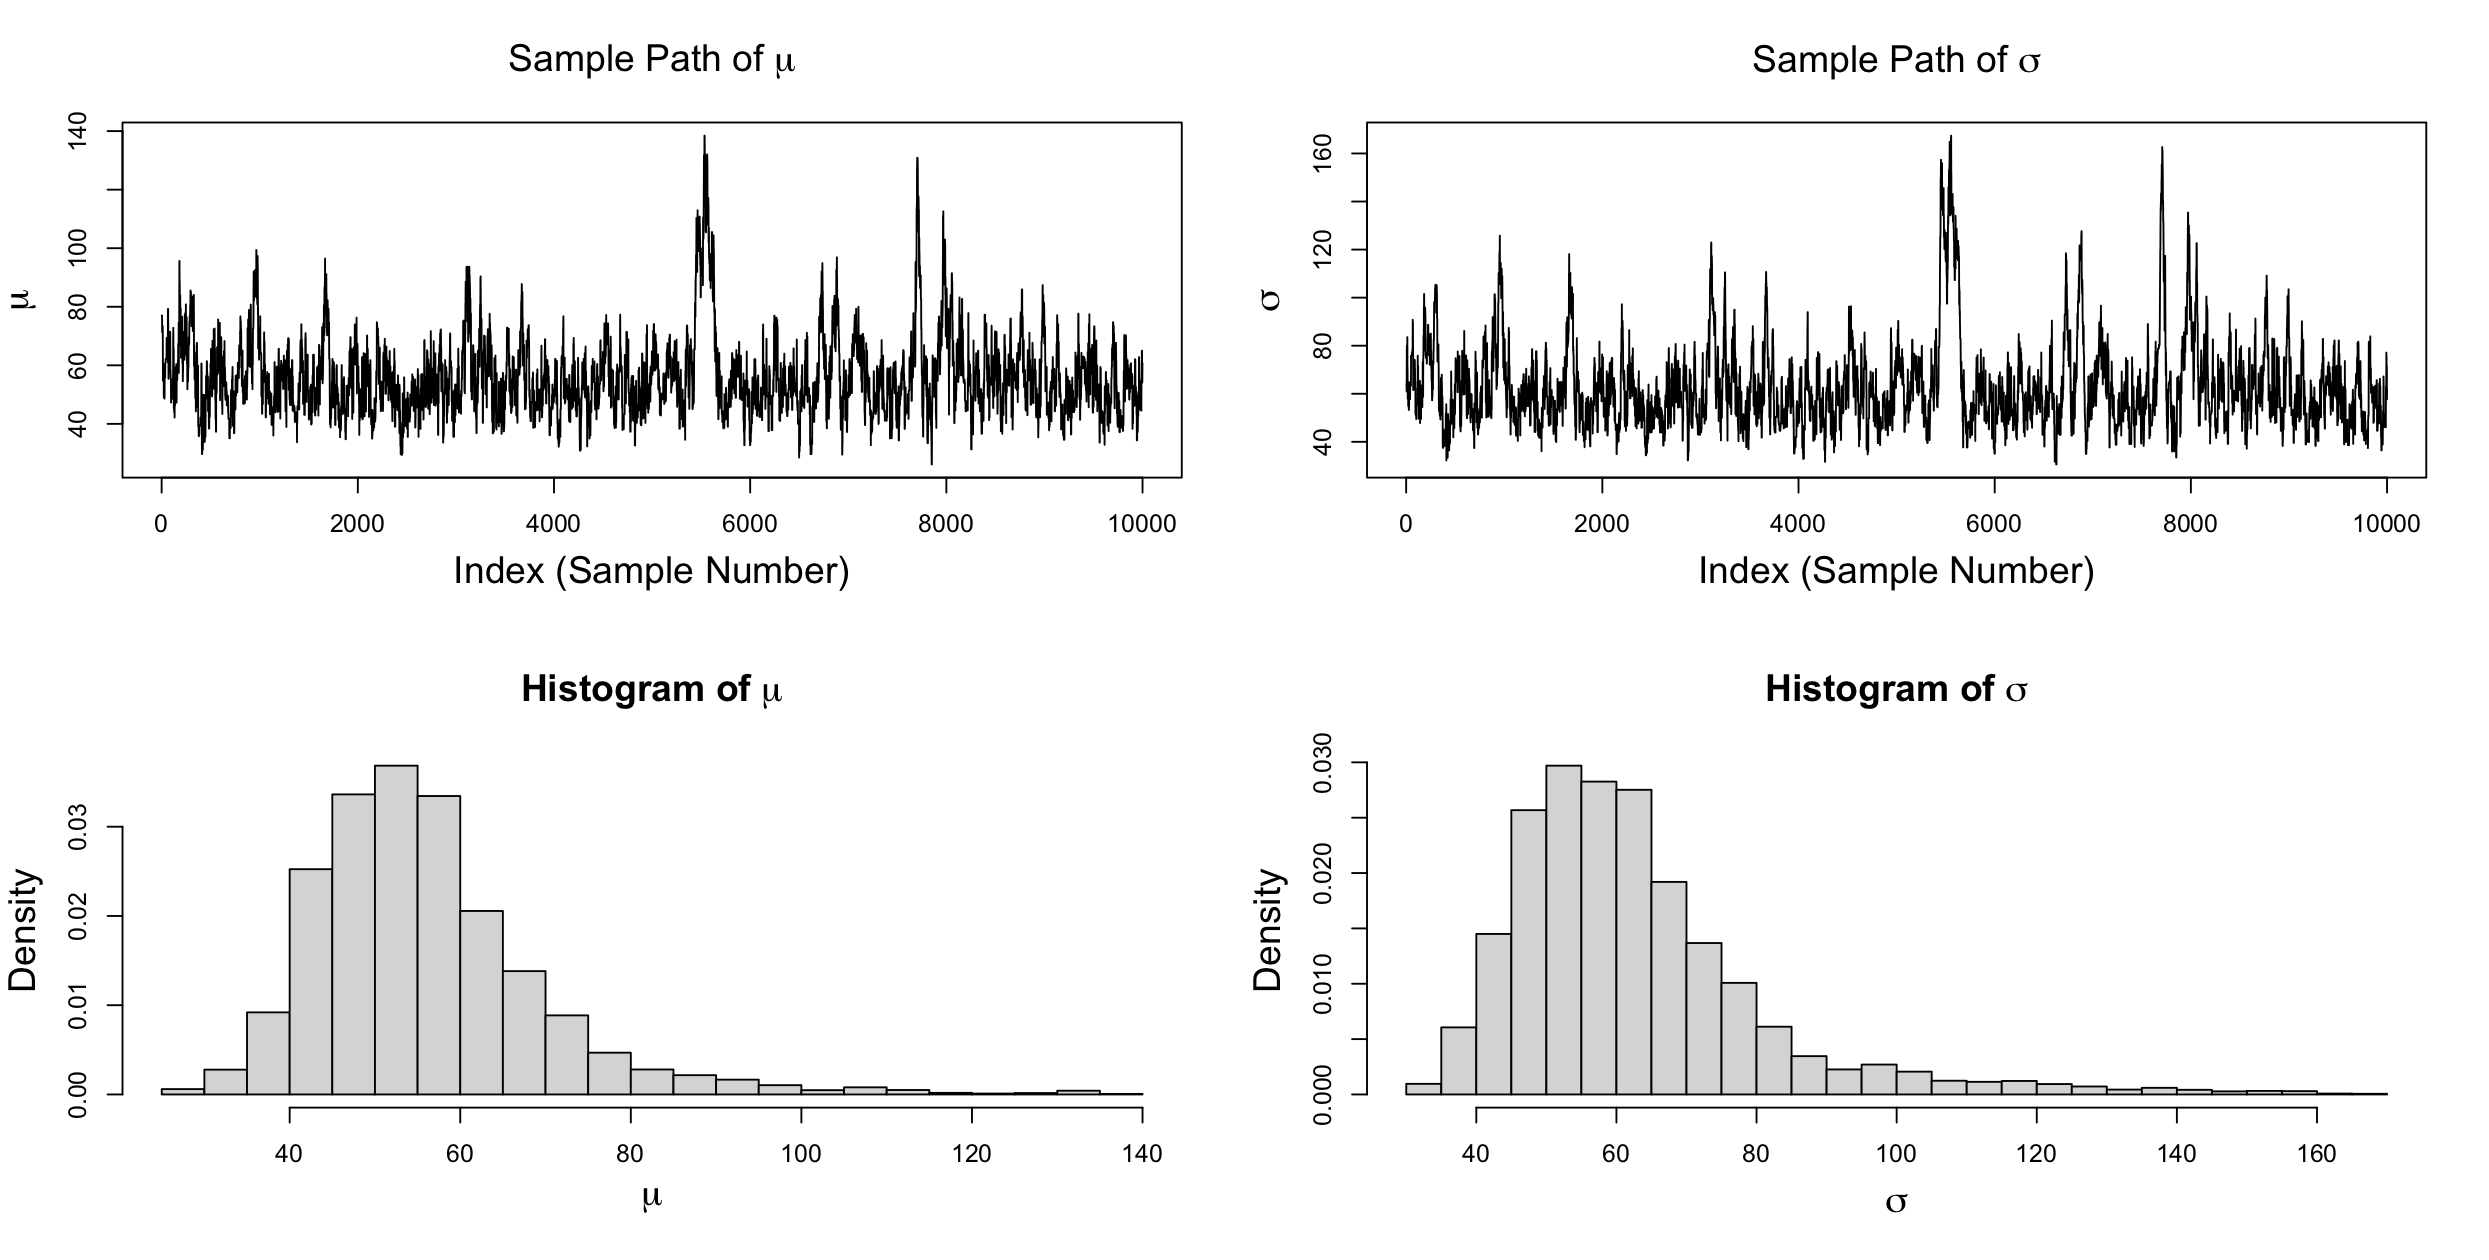
\includegraphics[width=6in,height=3.8in]{bayes_figs/Plots_mu_sigma.png} 
\end{figure}

In this case, $\hat{\tau}_{\text{int}}\approx50$ for each chain. This can be obtained using
\begin{verbatim}
1 + 2 * sum(abs(acf(mu, lag.max = 100, plot = F)$acf))     # tau_int for mu
[1] 48.50303
1 + 2 * sum(abs(acf(sigma, lag.max = 100, plot = F)$acf))  # tau_int for sigma
[1] 52.15097
\end{verbatim}
This means that those 10,000 MCMC samples are equivalent to only about 200 independent samples. It is usually the case that the chains are more correlated when we sample multiple parameters together.

There are lots of methods that can be used to reduce the autocorrelation in the chains like
\begin{itemize}
\item Changing the standard deviation of the proposal distributions.
\item Changing the proposal distribution altogether.
\item Using conjugate priors so Gibbs sampling can be used (Gibbs samples will usually lower autocorrelation than Metropolis samples).
\item Doing individual Metropolis sampling instead of the simultaneous ones we did here.
\item Use a different MCMC algorithm. There are lots of them!\\
\end{itemize}

\newpage

\fbox{\bf Regularization in the Bayesian Framework}

In Notes 7, we discussed regularization to add a bit of bias to an estimate in exchange for smaller variance. In ordinary least squares (OLS), we find the estimate for $\boldsymbol{\beta}$ by minimizing the sum of squared residuals. Therefore, we have 
\begin{align*}
\hat{\boldsymbol{\beta}}_{\text{OLS}}&=\underset{\boldsymbol{\beta}}{\arg\min}\left\{\sum_{i=1}^{n}\left(y_i-\sum_{j=0}^{p-1}x_{ij}\beta_j\right)^2\right\}\\
&=\underset{\boldsymbol{\beta}}{\arg\min}\left\{(\boldsymbol{y}-\boldsymbol{\beta})^T(\boldsymbol{y}-\boldsymbol{\beta})\right\}\\
&=\underset{\boldsymbol{\beta}}{\arg\min}\left\{\Vert\boldsymbol{y}-\boldsymbol{\beta}\Vert^2_2\right\},
\end{align*}
where $\Vert\cdot\Vert$ is the 2 norm. We saw with ridge regression, the estimates for the $\beta_i$ values for $i=1,\dots,p$, can be obtained using
\begin{align*}
\hat{\boldsymbol{\beta}}_{\text{ridge}}&=\underset{\boldsymbol{\beta}}{\arg\min}\left\{\sum_{i=1}^{n}\left(y_i-\sum_{j=0}^{p-1}x_{ij}\beta_j\right)^2+\lambda\sum_{j=1}^{p-1}\beta_j^2\right\}\\
&=\underset{\boldsymbol{\beta}}{\arg\min}\left\{(\boldsymbol{y}-\mathbf{X}\boldsymbol{\beta})^T(\boldsymbol{y}-\mathbf{X}\boldsymbol{\beta})+\lambda\boldsymbol{\beta}^T\boldsymbol{\beta}\right\}\\
&=\underset{\boldsymbol{\beta}}{\arg\min}\left\{\Vert\boldsymbol{y}-\mathbf{X}\boldsymbol{\beta}\Vert^2_2 + \lambda \Vert \boldsymbol{\beta}\Vert_2^2\right\}.
\end{align*}
In the Bayesian framework, we we a prior on $\boldsymbol{\beta}$ and a likelihood for $\boldsymbol{y}$. One of the assumptions of OLS is that $y_i|\mathbf{X}_i$ is normal and the $y_i$ values are independent. So, we have \\
$y_i|\mathbf{X}_i\sim N(\mathbf{X}_i\boldsymbol{\beta}, \sigma^2)$ where $\sigma$ is the variance of $y_i$. For all $y_i$ values, we have $\boldsymbol{y}\sim N(\mathbf{X}\boldsymbol{\beta}, \sigma^2 \mathbf{I})$ where $ \mathbf{I}$ is the identity matrix. Written another way, we can say 
$$
p(y_i|\mathbf{X}_i, \boldsymbol{\beta}) = \dfrac{1}{\sqrt{2\pi\sigma^2}}\exp\left\{-\frac{1}{2\sigma^2}(y_i-\mathbf{X}_i\boldsymbol{\beta})^2 \right\}\propto \exp\left\{-\frac{1}{2\sigma^2}(y_i-\mathbf{X}_i\boldsymbol{\beta})^2 \right\},
$$
which means
$$
p(\boldsymbol{y}|\mathbf{X}, \boldsymbol{\beta})\propto \exp\left\{-\frac{1}{2\sigma^2}(\boldsymbol{y}-\mathbf{X}\boldsymbol{\beta})^T(\boldsymbol{y}-\mathbf{X}\boldsymbol{\beta}) \right\}.
$$
Now, if we assign a normal prior for $\boldsymbol{\beta}$ and say $\boldsymbol{\beta}|\boldsymbol{y}, \mathbf{X}\sim N(0, \theta^2\mathbf{I})$, then the likelihood for $\boldsymbol{\beta}$ can be written
$$
p(\boldsymbol{\beta})\propto \exp\left\{-\frac{1}{2\theta^2}\boldsymbol{\beta}^T\boldsymbol{\beta} \right\}.
$$
That means the posterior will be found by multiplying:
\begin{align*}
	p(\boldsymbol{\beta}|\boldsymbol{y}, \mathbf{X})&\propto p(\boldsymbol{y}|\mathbf{X}, \boldsymbol{\beta})p(\boldsymbol{\beta})\\
	&\propto \exp\left\{-\frac{1}{2\sigma^2}(\boldsymbol{y}-\mathbf{X}\boldsymbol{\beta})^T(\boldsymbol{y}-\mathbf{X}\boldsymbol{\beta})\right\}
	\exp\left\{-\frac{1}{2\theta^2}\boldsymbol{\beta}^T\boldsymbol{\beta} \right\}\\
	&\propto \exp\left\{-\frac{1}{2\sigma^2}(\boldsymbol{y}-\mathbf{X}\boldsymbol{\beta})^T(\boldsymbol{y}-\mathbf{X}\boldsymbol{\beta})-\frac{1}{2\theta^2}\boldsymbol{\beta}^T\boldsymbol{\beta} \right\}.
\end{align*}

Then, to obtain the estimate for $\boldsymbol{\beta}$, we can maximize this posterior distribution. This is known as the maximum a posteriori (MAP) estimate. Notice that the $\boldsymbol{\beta}$ that maximizes this posterior is equivalent to minimizing the expression in the $\exp(\cdot)$ function without the negative signs:
\begin{align*}
	\hat{\boldsymbol{\beta}}_{\text{ridge}}&=\underset{\boldsymbol{\beta}}{\arg\min}\left\{\dfrac{1}{2\sigma^2}(\boldsymbol{y}-\mathbf{X}\boldsymbol{\beta})^T(\boldsymbol{y}-\mathbf{X}\boldsymbol{\beta})+\frac{1}{2\theta^2}\boldsymbol{\beta}^T\boldsymbol{\beta}\right\}\\
	&=\underset{\boldsymbol{\beta}}{\arg\min}\left\{(\boldsymbol{y}-\mathbf{X}\boldsymbol{\beta})^T(\boldsymbol{y}-\mathbf{X}\boldsymbol{\beta})+\frac{\sigma^2}{\theta^2}\boldsymbol{\beta}^T\boldsymbol{\beta}\right\}\\
	&=\underset{\boldsymbol{\beta}}{\arg\min}\left\{(\boldsymbol{y}-\mathbf{X}\boldsymbol{\beta})^T(\boldsymbol{y}-\mathbf{X}\boldsymbol{\beta})+\lambda\boldsymbol{\beta}^T\boldsymbol{\beta}\right\}
\end{align*}
where $\lambda=\dfrac{\sigma^2}{\theta^2}$. Therefore, assigning a normal prior with zero mean on $\boldsymbol{\beta}$ in the Bayesian framework is equivalent to ridge regression. We would have to change the prior to what is known as the Laplacian distribution for a LASSO.

Everything presented here is just scratching the surface of Bayesian methods!

%\fbox{\bf Naive Bayes Classifier} Save for SVM notes.


\end{document}  